\documentclass[10pt, colorlinks]{beamer}
  % compress
  %\documentclass[handout,xcolot=pdftex,dvipsnames,table]{beamer}
\definecolor{mybg}{RGB}{255,255,204}
\usepackage{minted}
\usepackage{graphicx}
\usepackage[english]{babel}
\usepackage[utf8x]{inputenc}
%\usepackage{amsmath}


 % \usepackage{beamerthemesplit}

%\usemintedstyle{trac}

\mode<presentation>
\setbeamercovered{invisible}
\usetheme{Warsaw}
\usecolortheme{dolphin}

\usefonttheme{serif}



\title{ Python in a Nutshell}
\subtitle
 {Part IV: Scikits } % (optional)


\author[Velasco and Perera]{Manel Velasco,\inst{1} PhD and Alexandre Perera,\inst{1}$^{,}$\inst{2} PhD}

\institute[UPC] % (optional, but mostly needed)
{
  \inst{1}%
  Departament d'Enginyeria de Sistemes, Automatica i Informatica Industrial (ESAII)  \\
  Universitat Politecnica de Catalunya 
  \and 
  \inst{2}%
   Centro de Investigacion Biomedica en Red en Bioingenieria, Biomateriales y Nanomedicina (CIBER-BBN)  \\
    \href{mailto:Alexandre.Perera@upc.edu}{Alexandre.Perera@upc.edu}~\href{mailto:manel.velasco@upc.edu}{Manel.Velasco@upc.edu}
}
 

\date[Feb, 2013, Learning Python]{Introduction to Python for Engineering and Statistics\\
Febraury, 2013}

 %

\begin{document}


\begin{frame}[plain]
   %  \titlepage
   \maketitle
\end{frame}

\begin{frame}[allowframebreaks]{Contents}
  \tableofcontents
  % You might wish to add the option [pausesections]
 \note[options]{aixo son notes}
\end{frame}

%----------------------------FRAME------------------------------------
\begin{frame}[fragile]\frametitle{Machine Learning}
\begin{figure}[!htb]
    \centering
    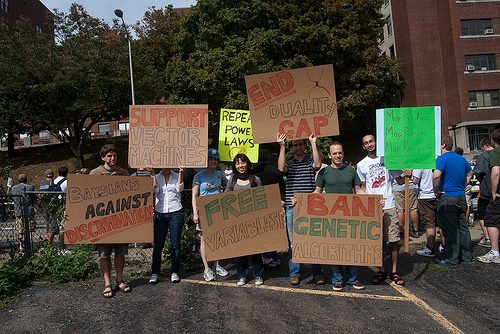
\includegraphics[width=0.8\textwidth]{figs/machine}
\end{figure}
\end{frame}



\section{Introduction to Python Scikits}
%----------------------------FRAME------------------------------------
\begin{frame}[fragile]\frametitle{Scikits}

\begin{itemize}
    \item SciKits (short for SciPy Toolkits), are add-on packages for SciPy, hosted and developed separately from the main SciPy distribution.
    \item The SciKits cover a broad spectrum of application domains, including financial computation, audio processing, geosciences, computer vision, engineering, machine learning, medical computing and bioinformatics.
    \item All SciKits are available under the 'scikits' namespace and are licensed under OSI-approved licenses.
    \item Packages are packaged as toolkits (instead of in the main, monolithic SciPy distribution) when:
\begin{enumerate}
    \item The package is deemed too specialized to live in SciPy itself or

    \item The package has a GPL (or similar) license which is incompatible with SciPy's BSD license or

    \item The package is meant to be included in SciPy, but development is still in progress.
\end{enumerate}
\end{itemize}
\end{frame}

%----------------------------FRAME------------------------------------
\begin{frame}[fragile]\frametitle{Scikits}

\begin{block}{Avaliable kits}
The list of available kits can be found at  \\ 
    \centering \href{http://scikits.appspot.com/scikits}{http://scikits.appspot.com/scikits}.
\end{block}

\end{frame}

%----------------------------FRAME------------------------------------
\begin{frame}[fragile]\frametitle{Scikits}
\begin{block}{Main scikits}
\begin{description}
    \item[scikit-aero]  Aeronautical engineering calculations in Python.
    \item[scikit-image] Image processing routines for SciPy.
    \item[scikit-rf] Object Oriented Microwave Engineering.
    \item[audiolab] A python module to make noise from numpy arrays (sic).
    \item[timeseries] Time series manipulation.
    \item[learn] Machine learning Sci-kit. 
\end{description}
\end{block}

\end{frame}

\subsection{pandas} % (fold)
\label{sec:scikit timeseries}



%----------------------------FRAME------------------------------------
\begin{frame}[fragile]\frametitle{pandas}
\begin{block}{timeseries}
The scikits.timeseries module is no longer undergoing active development. There is an outstanding list of bugs that are unlikely to be fixed. The plan is for the core functionality of this module to be implemented in pandas.
\end{block}
\end{frame}
%----------------------------FRAME------------------------------------
\begin{frame}[fragile]\frametitle{pandas}
\begin{block}{Python Data Analysis Library (pandas)}
Python has long been great for data munging and preparation, but less so for data analysis and modeling. \emph{pandas} helps fill this gap, enabling you to carry out your entire data analysis workflow in Python without having to switch to a more domain specific language like R.
\end{block}

\end{frame}
%----------------------------FRAME------------------------------------
\begin{frame}[fragile]\frametitle{pandas features}
\begin{block}{pandas features}
\begin{itemize}
    \item A fast and efficient DataFrame object for data manipulation with integrated indexing.
    \item Tools for reading and writing data between in-memory data structures and different formats: CSV and text files, Microsoft Excel, SQL databases, and the fast HDF5 format.
    \item Intelligent data alignment and integrated handling of missing data: gain automatic label-based alignment in computations and easily manipulate messy data into an orderly form.
    \item High performance merging and joining of data sets.
\end{itemize}
\end{block}

\end{frame}
%----------------------------FRAME------------------------------------
\begin{frame}[fragile]\frametitle{pandas}
\small
\begin{minted} [bgcolor=mybg,frame=lines,bgcolor=mybg,frame=lines,bgcolor=mybg,frame=lines,mathescape]{python}
In [1]: index = date_range('1/1/2000', periods=8)

In [2]: s = Series(randn(5), index=['a', 'b', 'c', 'd', 'e'])

In [3]: df = DataFrame(randn(8, 3), index=index,
   ...:                columns=['A', 'B', 'C'])
   ...:

In [4]: wp = Panel(randn(2, 5, 4), items=['Item1', 'Item2'],
   ...:            major_axis=date_range('1/1/2000', periods=5),
   ...:            minor_axis=['A', 'B', 'C', 'D'])
   ...:
\end{minted}

\end{frame}

%----------------------------FRAME------------------------------------
\begin{frame}[fragile]\frametitle{pandas}
\begin{minted} [bgcolor=mybg,frame=lines,bgcolor=mybg,frame=lines,bgcolor=mybg,frame=lines,mathescape]{python}
In [39]: df
Out[39]: 
        one     three       two
a  2.213700       NaN -1.436616
b  0.115002  0.640476 -1.107900
c  0.008462  0.697707  0.844137
d       NaN  0.331810 -0.429735

In [40]: df.mean(0)
Out[40]: 
one      0.779055
three    0.556664
two     -0.532528

\end{minted}

\end{frame}

% section scikit timeseries (end)
%
\subsection{audiolab} % (fold)
\label{sec:audiolab}
%----------------------------FRAME------------------------------------
\begin{frame}[fragile]\frametitle{audiolab}
\begin{block}{audiolab}
Is essentially a  wrapper around Erik de Castro Lopo's excellent libsndfile:\\
    \centering \href{http://www.mega-nerd.com/libsndfile/}{http://www.mega-nerd.com/libsndfile/} 
\end{block}
\small
\begin{block}{}
Audiolab is a python package to read/write audio files from numpy arrays. Matlab have functions such as wavread, wavwrite, soundsc, etc. Main features are:
\begin{itemize}
    \item Reading all formats supported by sndfile directly into numpy arrays.
    \item Writing all formats supported by sndfile directly from numpy arrays.
    \item A matlab-like API (e.g. wavread) for some file formats. Wav, aiff, flac, au, and ogg formats are supported.
    \item A play function to output data from numpy array into the sound device of your computer (Only ALSA for linux and CoreAudio for Mac OS X is implemented ATM).
\end{itemize}
\end{block}

\end{frame}

%----------------------------FRAME------------------------------------
\begin{frame}[fragile]\frametitle{audiolab overview}
\small \begin{minted} [bgcolor=mybg,frame=lines,bgcolor=mybg,frame=lines,bgcolor=mybg,frame=lines,mathescape]{python}
from audiolab import wavread
data, fs, enc = wavread('test.wav')
import numpy as np
from scikits.audiolab import Sndfile

f = Sndfile('test.wav', 'r')

# Sndfile instances can be queried for the audio file meta-data
fs = f.samplerate
nc = f.channels
enc = f.encoding

# Reading is straightforward
data = f.read_frames(1000)

# This reads the next 1000 frames, e.g. from 1000 to 2000,
# but as single precision
data_float = f.read_frames(1000, dtype=np.float32)
\end{minted}

\end{frame}

%----------------------------FRAME------------------------------------
\begin{frame}[fragile]\frametitle{audiolab}

\small \begin{minted} [bgcolor=mybg,frame=lines,bgcolor=mybg,frame=lines,bgcolor=mybg,frame=lines,mathescape]{python}
import numpy as np
from scikits.audiolab import Format, Sndfile

filename = 'foo.wav'

# Create some data to save as audio data: one 
# second of stereo white noise
data = np.random.randn(48000, 2)

# Create a Sndfile instance for writing wav files @ 48000 Hz
format = Format('wav')
f = Sndfile(filename, ' w', format, 2, 48000)

# Write the first 500 frames of the signal. 
# Note that the write_frames method
# uses tmp's numpy dtype to determine how to 
# write to the file; sndfile also
# converts the data on the fly if necessary
f.write_frames(data[:500]); f.close()
\end{minted}

\end{frame}
%----------------------------FRAME------------------------------------
\begin{frame}[fragile]\frametitle{audiolab}
\begin{minted} [bgcolor=mybg,frame=lines,bgcolor=mybg,frame=lines,bgcolor=mybg,frame=lines,mathescape]{python}
import numpy as np
from scikits.audiolab import play

# output one second of stereo 
#    gaussian white noise at 48000 hz

play(0.05 * np.random.randn(2, 48000))
\end{minted}


\end{frame}

% section audiolab (end)


\section{scikit-learn} % (fold)
\label{sec:scikit-learn}

\subsection{Datasets in sklearn} % (fold)
\label{sub:Datasets in sklearn}

% subsection Datasets in sklearn (end)
%----------------------------FRAME------------------------------------
\begin{frame}[fragile]\frametitle{Introduction}
\begin{block}{Datasets}
There are three different datasets in sklearn:
\begin{enumerate}
    \item Sample images.
    \item Toy Datasets.
    \item Sample Generators.
\end{enumerate}
\end{block}
\end{frame}
%----------------------------FRAME------------------------------------
\begin{frame}[fragile]\frametitle{Image sets}
The scikit also embed a couple of sample JPEG images (china and flower) published under Creative Commons license by their authors.
\begin{columns}[c]
\column{0.6\textwidth}

%-------------------------------CODE
\small
\begin{minted}[bgcolor=mybg,frame=lines,mathescape]{python}
import numpy as np
import pylab as pl
from sklearn.datasets import load_sample_image
china = load_sample_image("china.jpg")
\end{minted}

%-------------------------------END CODE
\column{0.4\textwidth}
%-------------------------------CODE
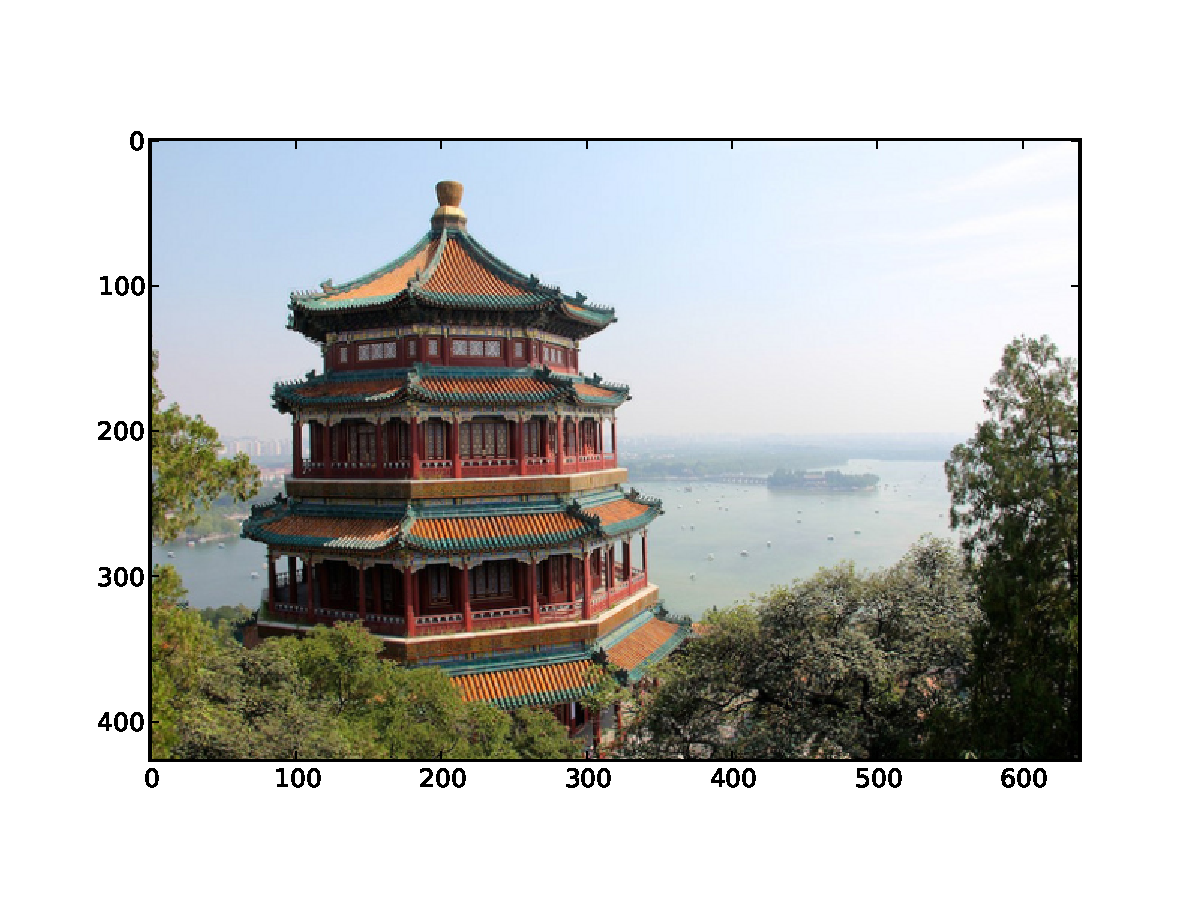
\includegraphics[width=\textwidth]{plwfigis/CursP_4_figure2}

%-------------------------------END CODE
\end{columns}

\end{frame}

%----------------------------FRAME------------------------------------
\begin{frame}[fragile]\frametitle{Toy datasets}
\begin{description}
    \item[load\_boston()] \textcolor{green}{Regression} Load and return the boston house-prices dataset.
    \item[load\_iris()] \textcolor{red}{Classification} Load and return the iris dataset.
    \item[load\_diabetes()] \textcolor{green}{Regression} Load and return the diabetes dataset.
    \item[load\_iris()] \textcolor{red}{Classification} Load and return the digits dataset.
     \item[load\_linnerud()] \textcolor{green}{Multivariate Regression} 	Load and return the linnerud dataset.
\end{description}
These functions return a \emph{bunch} (which is a dictionary that is accessible with the \emph{dict.key} syntax). All datasets have at least two keys, 
\begin{itemize}
    \item \textcolor{red}{data}, containing an array of shape $n$ samples $\times$ $n$ features and 
    \item \textcolor{red}{target}, a numpy array of length $n$ features, containing the targets.
\end{itemize}
\end{frame}

%----------------------------FRAME------------------------------------
\begin{frame}[fragile]\frametitle{Data Generators}
A number of functions exists to create the most esoteric data distributions: 
\begin{description}
    \item[make\_classification()] n-class classification problem (+ multilabel).
    \item[make\_regression()] Generate a regression problem.
    \item[make\_swiss\_roll()] Generate swiss roll datasets.
    \item[make\_s\_curve]  Generates S curve datasets.
\end{description}
All of them returning a tuple $(X, y)$ consisting of a $n$ samples $\times$ $n$ features numpy array $X$ and an array of length $n$ samples containing the targets $y$.

\end{frame}



%----------------------------FRAME------------------------------------
\begin{frame}[fragile]\frametitle{Data Generators}
\begin{figure}[!htb]
    \centering
    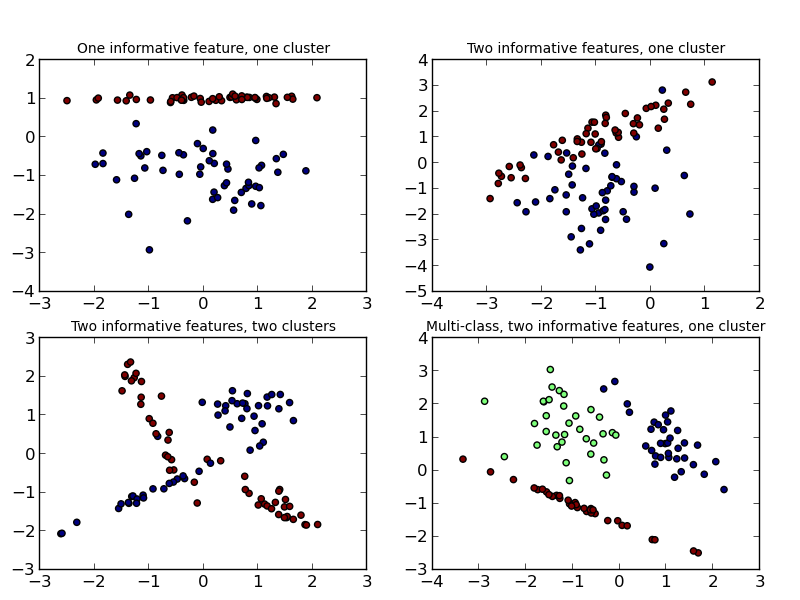
\includegraphics[width=0.85\textwidth]{figs/randomdata}
\end{figure}
\end{frame}

%----------------------------FRAME------------------------------------
\begin{frame}[fragile]\frametitle{Challenge}

\begin{block}{5 mins challenge}
Generate and plot a dataset with two non-overlapping swiss rolls on $\mathbb{R}^3$ with 1000 samples each.  
\end{block}
Tip, you can generate a rotation matrix with help of this function: 

%-------------------------------CODE
\begin{minted}[bgcolor=mybg,frame=lines,mathescape]{python}
import numpy as np
def rot(angle, R = np.zeros((3,3))):
    cx, cy, cz = np.cos(angle)
    sx, sy, sz = np.sin(angle)
    R.flat = (cx*cz -sx*cy*sz, cx*sz + sx*cy*cz, sx*sy,\
     -sx*cz - cx*cy*sz, -sx*sz +cx*cy*cz, cx*sy,\
     sy*sz, -sy*cz, cy)
    return R
\end{minted}

%-------------------------------END CODE

%-------------------------------END CODE
\end{frame}

%----------------------------FRAME 2 cols------------------------------
\begin{frame}[fragile]\frametitle{}
\begin{columns}[c]
\column{\textwidth}
%-------------------------------CODE
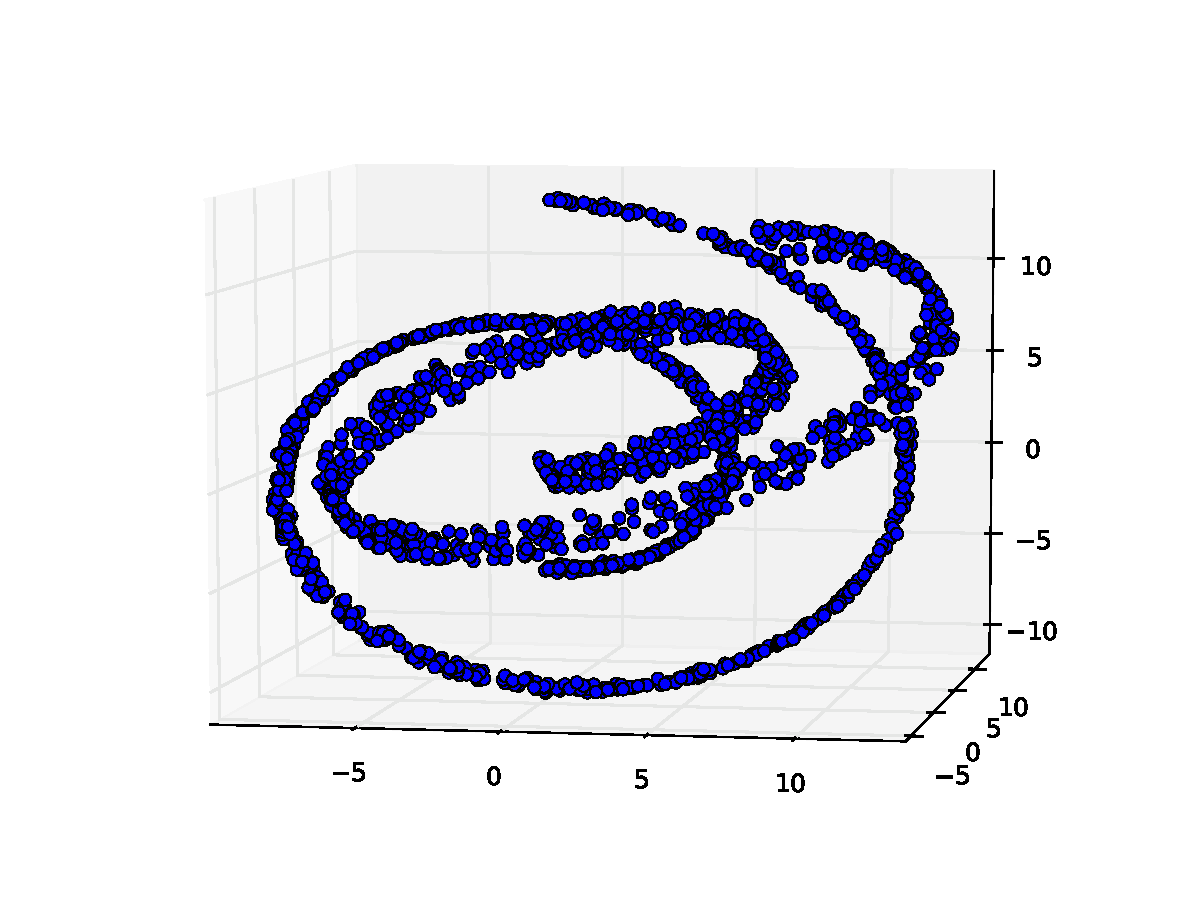
\includegraphics[width=\textwidth]{plwfigis/CursP_4_figure4}

%-------------------------------END CODE

\end{columns}
\end{frame}

\subsection{Unsupervised Learning} % (fold)
\label{sec:Clustering}


%----------------------------FRAME------------------------------------
\begin{frame}[fragile]\frametitle{Introduction to clustering in python}
\begin{block}{Clustering}
Or Cluster Analysis, is the task of grouping a set of objects in such a way that objects in the same groups (clusters) are more similar to each other than to those in other groups.
\end{block}
It is useful in a large amount of applications:
   \begin{itemize}
       \item Exploratory analysis.
        \item Machine Learning \& Pattern Recognition.
        \item Image analysis.
        \item Bioinformatics.
        \item Market Analysis.
   \end{itemize}
\end{frame}


%----------------------------FRAME------------------------------------
\begin{frame}[fragile]\frametitle{Clustering}
\begin{center}
    
\only<1>{\centering  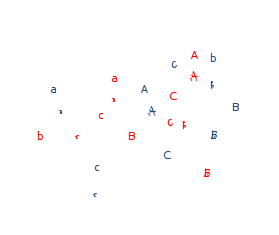
\includegraphics[scale=0.8]{figs/similitude/Slide1} }
\only<2>{\centering  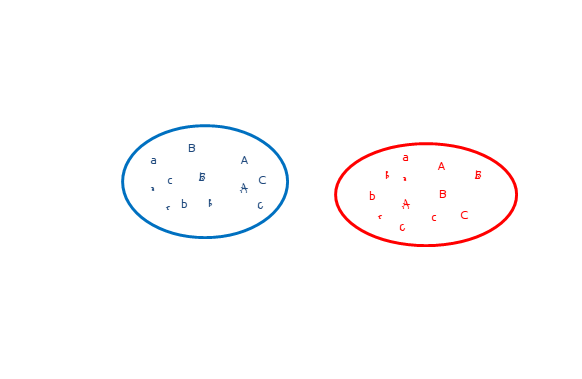
\includegraphics[scale=0.7]{figs/similitude/Slide4} }
\only<3>{\centering  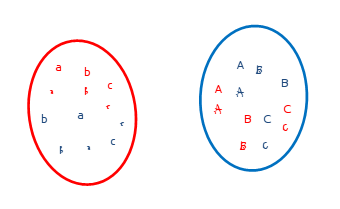
\includegraphics[scale=0.8]{figs/similitude/Slide5} }
\only<4>{\centering  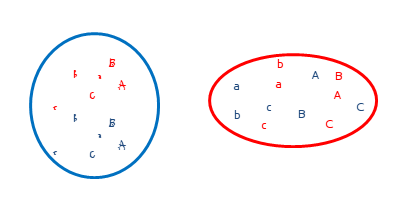
\includegraphics[scale=0.8]{figs/similitude/Slide3} }
\only<5>{\centering  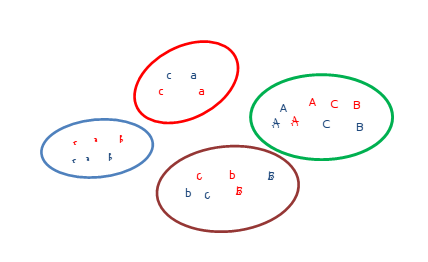
\includegraphics[scale=0.8]{figs/similitude/Slide2} }

\end{center}
\end{frame}


%----------------------------FRAME------------------------------------
\begin{frame}[fragile]\frametitle{Clustering algorithms in sklearn}
\begin{figure}[!htb]
    \centering
    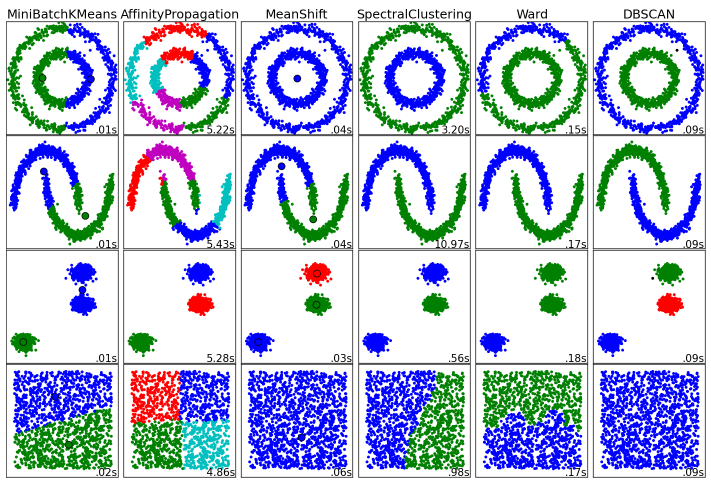
\includegraphics[width=0.9\textwidth]{figs/clustering}
\end{figure}
\end{frame}
%----------------------------FRAME------------------------------------
\begin{frame}[fragile]\frametitle{Notes on Clustering input}
\begin{block}{Input data formats}
One important thing to note is that the algorithms implemented in this module take different kinds of matrix as input.
    \begin{itemize}
    \item \textcolor{blue}{MeanShift and KMeans} take data matrices of shape [n\_samples, n\_features]. The are obtained from  \verb|sklearn.feature\_extraction| module. 
    \item \textcolor{blue}{AffinityPropagation and SpectralClustering} take similarity matrices of shape [n\_samples, n\_samples]. These are obtained from  \verb|sklearn.metrics.pairwise module|. 
    \end{itemize} 
\end{block}

\end{frame}

%----------------------------FRAME------------------------------------
\begin{frame}[fragile]\frametitle{sklearn.metrics.pairwise}
\begin{block}{sklearn.metrics.pairwise}
Contains both distances and kernels. There are a number of ways to convert between a distance metric and a similarity measure, such as a kernel. Let $D$ be the distance, and $S$ be the kernel:
\begin{align}
    s(x,y) &= e^{-d(x,y) \over \gamma } \\
    s(x,y) &= \frac{1}{\frac{d(x,y)}{max(D)}} 
\end{align}
\end{block}
\pause
\begin{block}{sklearn.metrics.pairwise.rbf\_kernel(X, Y=None, gamma=0)}
Compute the rbf (gaussian) kernel between X and Y:
\begin{equation}
    K(x,y) = e^{-\gamma ||x-y||^2}
\end{equation}
\end{block}

\end{frame}




%----------------------------FRAME 2 cols------------------------------
\begin{frame}[fragile]\frametitle{{Learning Clustering in python}}
\begin{columns}[c]
\column{0.5\textwidth}
Let's recover our previous challenge (the two swiss rolls). 

\begin{block}{}
Could we automagically assign each sample to an egg roll?  Open your ipython and:
\begin{itemize}
    \item Use first k-means.
    \item Try another clustering algorithm.
\end{itemize}
\end{block}

\column{0.5\textwidth}
%-------------------------------CODE
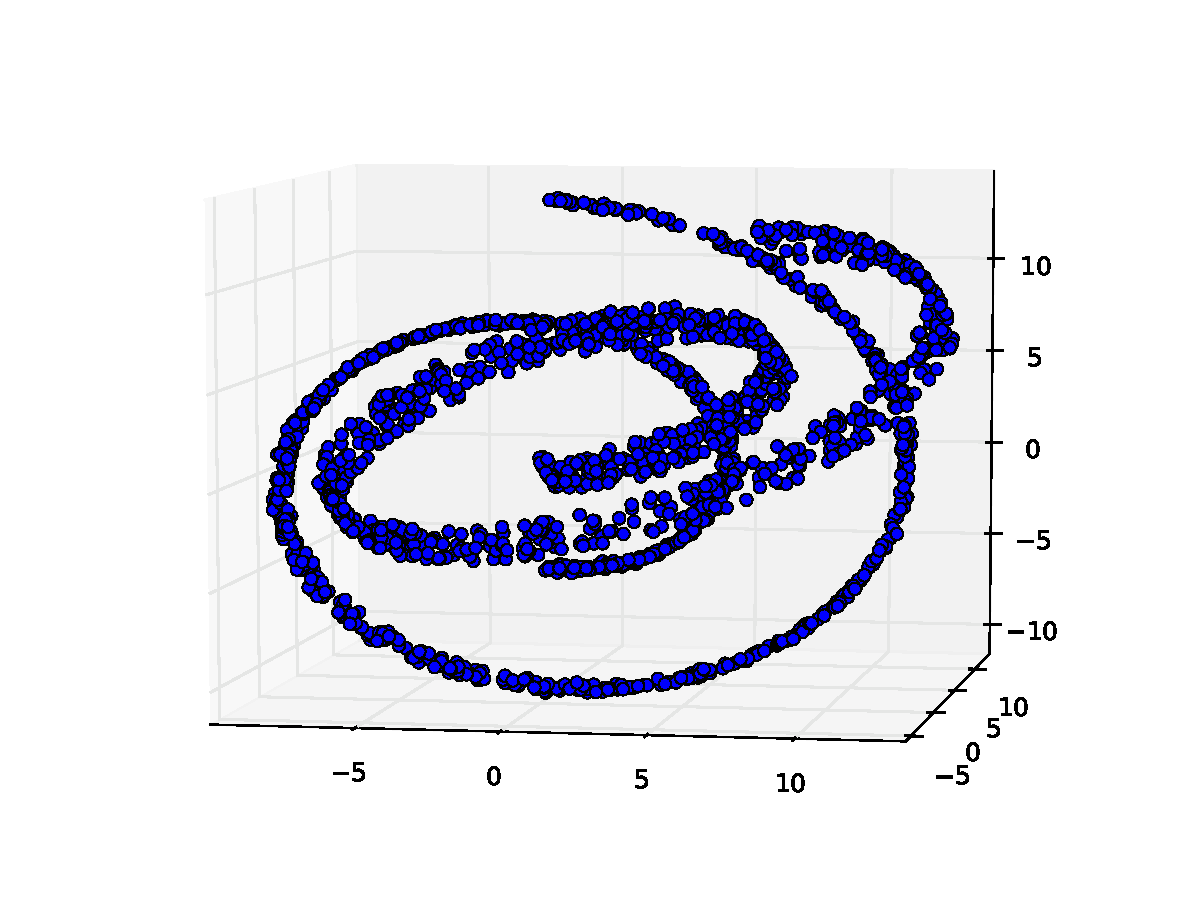
\includegraphics[width=\textwidth]{plwfigis/CursP_4_figure5}

%-------------------------------END CODE
\end{columns}
\end{frame}

\subsection{Principal Component Analysis} % (fold)
\label{sec:}
%----------------------------FRAME 2 cols + header (box)-------------
\begin{frame}[fragile]\frametitle{Principal Components Analysis}
\begin{block}{PCA}
PCA is an orthogonal linear transformation that creates a data model with a new coordinate system with a criteria for maximum variance captured.
 \begin{equation}
     w_1 = \arg\max_{||w||=1} \left\{ E(w^T X)^2\right\}
 \end{equation}
\end{block}
\end{frame}


\begin{frame}
  \frametitle{Principal Component Analysis }
  \begin{block}{}
    Most popular and commonly used methods. Sometimes included in the
    ``Factor Analysis'' methods.
  \end{block}
  \begin{itemize}
  \item<+-> It's the second most main tool for visualization
    \begin{itemize}
    \item (First is always to plot the signals!)
    \end{itemize}
  \item<+-> Main goal of PCA is to capture main directions of variance
    in input space.
  \item<+-> Dimensionality reduction:
    \begin{itemize}
    \item<+-> Allows for projecting the dataset onto a low dimensional subspace.
    \item<+-> Form of compression, or data modeling.
    \item<+-> Filtering.
    \end{itemize}

  \end{itemize}
\end{frame}



\begin{frame}
    \frametitle{Principal Component Analysis }
    \begin{center}
        \centering 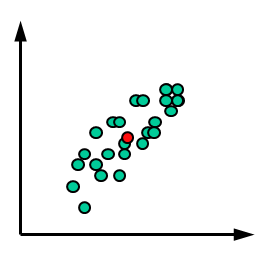
\includegraphics[width=0.6\textwidth]{figs/center}
    \end{center}  

\end{frame}

\begin{frame}
    \frametitle{Principal Component Analysis }
    
    \begin{center}
        \centering 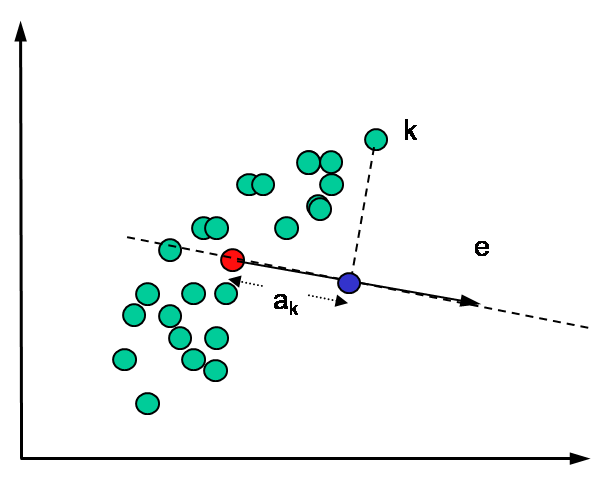
\includegraphics[width=0.6\textwidth]{figs/pca1}
    \end{center}        
    
\end{frame}


\begin{frame}
    \frametitle{PCA }
    \begin{center}
        \centering 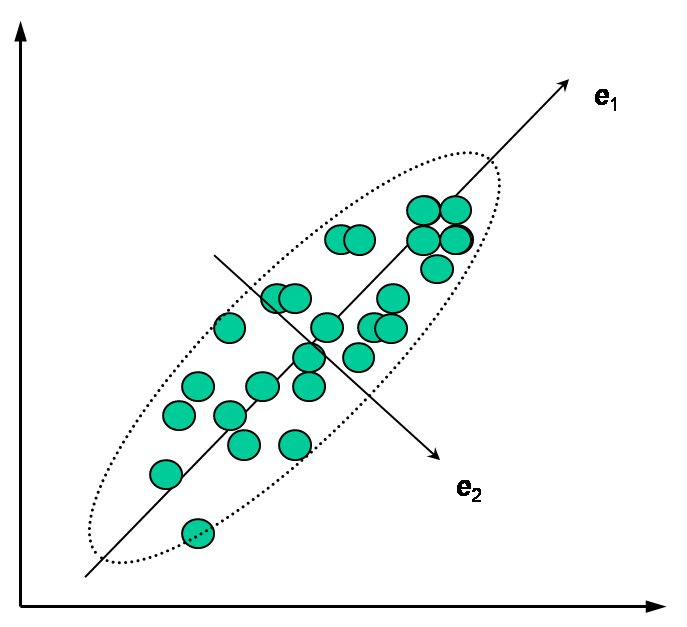
\includegraphics[width=0.6\textwidth]{figs/pca2}
    \end{center}
\end{frame}

 


\begin{frame}
    \frametitle{PCA }
    \begin{center}
        \centering 
\includegraphics[width=\textwidth]{figs/pca3}
    \end{center}
    \begin{columns}
        \pause      \begin{column}{0.3\textwidth}
            \begin{center}
                \centering 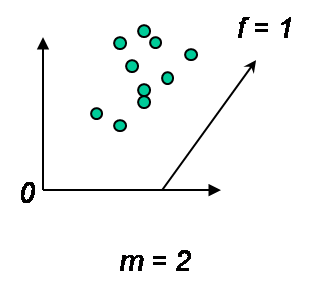
\includegraphics[width=\columnwidth]{figs/pcab1}
            \end{center}            
        \end{column}
        \pause         \begin{column}{0.3\textwidth}
            \begin{center}
                \centering 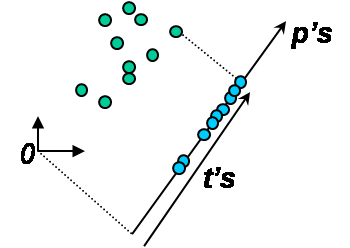
\includegraphics[width=\columnwidth]{figs/pcab2}
            \end{center}            
        \end{column}
        \pause         \begin{column}{0.3\textwidth}
            \begin{center}
                \centering 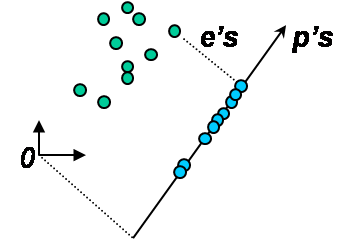
\includegraphics[width=\columnwidth]{figs/pcab3}
            \end{center}            
        \end{column}     
    \end{columns}
\end{frame}

%----------------------------FRAME 2 cols + header (box)-------------
\begin{frame}[fragile]\frametitle{The Iris dataset}
\begin{block}{Iris dataset}
The iris dataset is a classical classification task consisting in identifying 3 different types of irises (Setosa, Versicolour, and Virginica) from their petal and sepal length and width.
\end{block}
\begin{columns}[c]
\column{0.5\textwidth}
%-------------------------------CODE
\small
\begin{minted}[bgcolor=mybg,frame=lines,mathescape]{python}
>>> import numpy as np
>>> from sklearn import datasets
>>> import matplotlib.pylab as pl
>>> iris = datasets.load_iris()
>>> X = iris.data
>>> y = iris.target
>>> X[:2,:]
array([[ 5.1,  3.5,  1.4,  0.2],
       [ 4.9,  3. ,  1.4,  0.2]])
>>> np.unique(y)
array([0, 1, 2])
\end{minted}

%-------------------------------END CODE
\column{0.5\textwidth}
%-------------------------------CODE
\begin{minted}[bgcolor=mybg,frame=lines,mathescape]{python}
pl.scatter(X[:, 0], X[:, 1],
     c=y)
pl.xlabel('Sepal length')
pl.ylabel('Sepal width')
\end{minted}

%-------------------------------END CODE
\end{columns}
\end{frame}

%----------------------------FRAME------------------------------------
\begin{frame}[fragile]\frametitle{Iris Dataset}
\begin{columns}[c]
\column{0.4\textwidth}
    \centering
    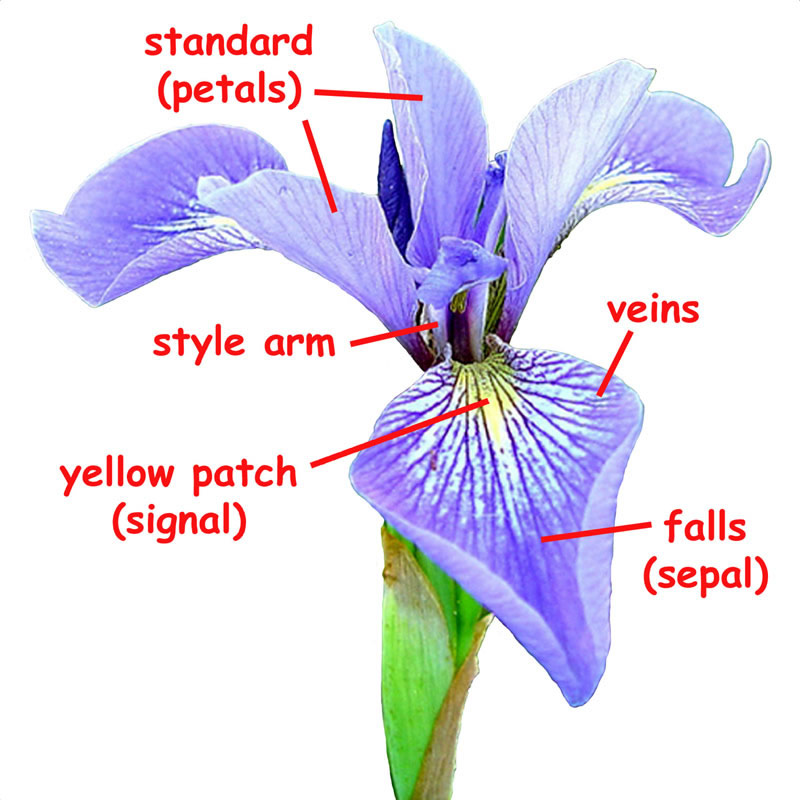
\includegraphics[width=\textwidth]{figs/iris}
\column{0.6\textwidth}

%-------------------------------CODE
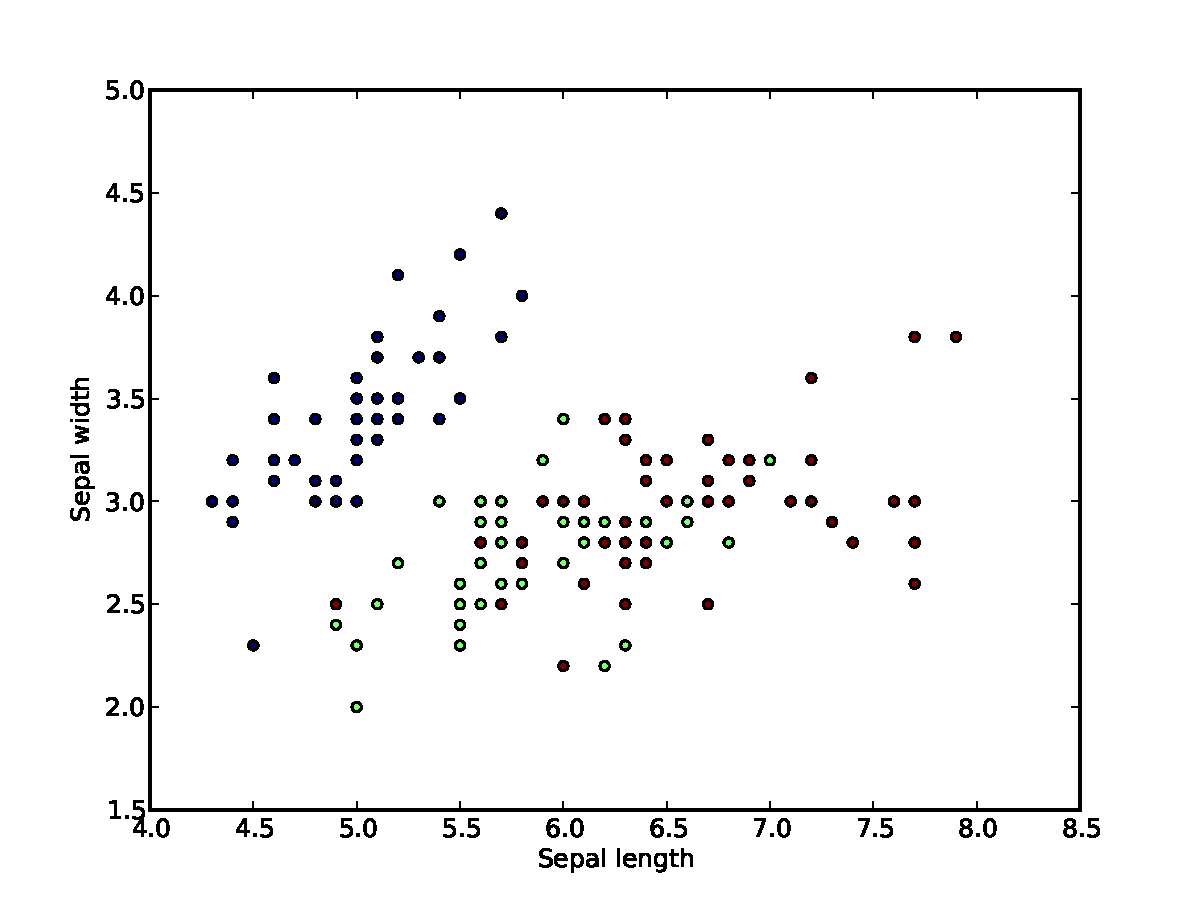
\includegraphics[width=\textwidth]{plwfigis/CursP_4_figure8}

%-------------------------------END CODE
\end{columns}
\end{frame}


%----------------------------FRAME------------------------------------
\begin{frame}[fragile]\frametitle{PCA in python }
It's very easy now to construct the PCA projection:
%-------------------------------CODE
\begin{minted}[bgcolor=mybg,frame=lines,mathescape]{python}
>>> from sklearn import decomposition
>>> pca = decomposition.PCA(n_components=2)
>>> pca.fit(X)
PCA(copy=True, n_components=2, whiten=False)
>>> T = pca.transform(X)
\end{minted}

%-------------------------------END CODE
\end{frame}

%----------------------------FRAME 2 cols------------------------------
\begin{frame}[fragile]\frametitle{PCA in python}

\begin{columns}[c]
\column{0.5\textwidth}
%-------------------------------CODE
\begin{minted}[bgcolor=mybg,frame=lines,mathescape]{python}
import pylab as pl
pl.scatter(T[:, 0], T[:, 1], \
    c=y) 
pl.xlabel('1PC')
pl.ylabel('2PC')
\end{minted}

%-------------------------------END CODE
\column{0.5\textwidth}
%-------------------------------CODE
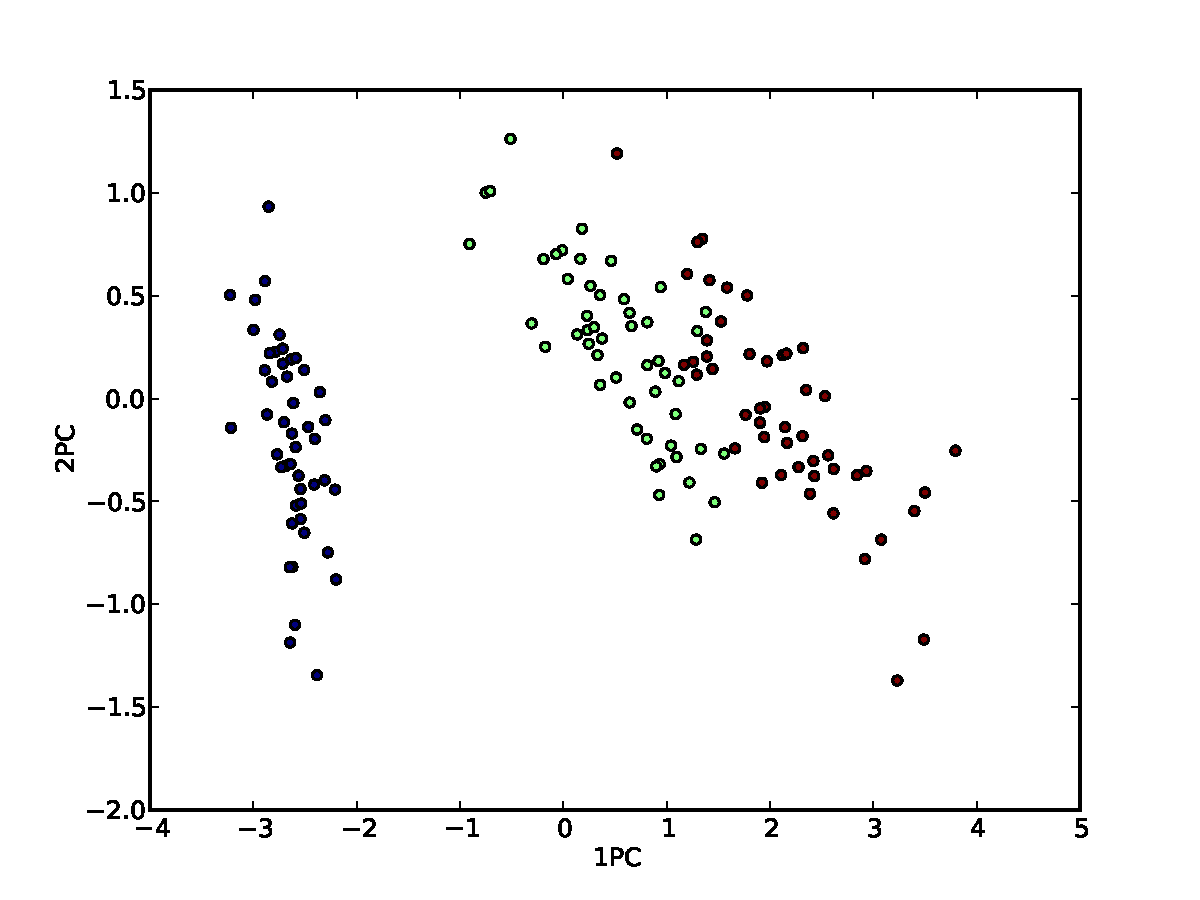
\includegraphics[width=\textwidth]{plwfigis/CursP_4_figure11}

%-------------------------------END CODE
\end{columns}
\end{frame}

% section  (end)

\subsection{Supervised Learning} % (fold)
\label{sec:Classfication}
%----------------------------FRAME------------------------------------
\begin{frame}[fragile]\frametitle{Supervised Learning}
\begin{block}{Supervised Learning}
Consists in learning the link between two datasets:
\begin{itemize}
    \item An observed data $X$ and
    \item  A variable $y$ usually called target or labels. 
\end{itemize}
\end{block}
\end{frame}





%----------------------------FRAME------------------------------------
\begin{frame}[fragile]\frametitle{Classification algorithms in sklearn}
\begin{center}
 \begin{figure}[!htb]
   
   
\centering    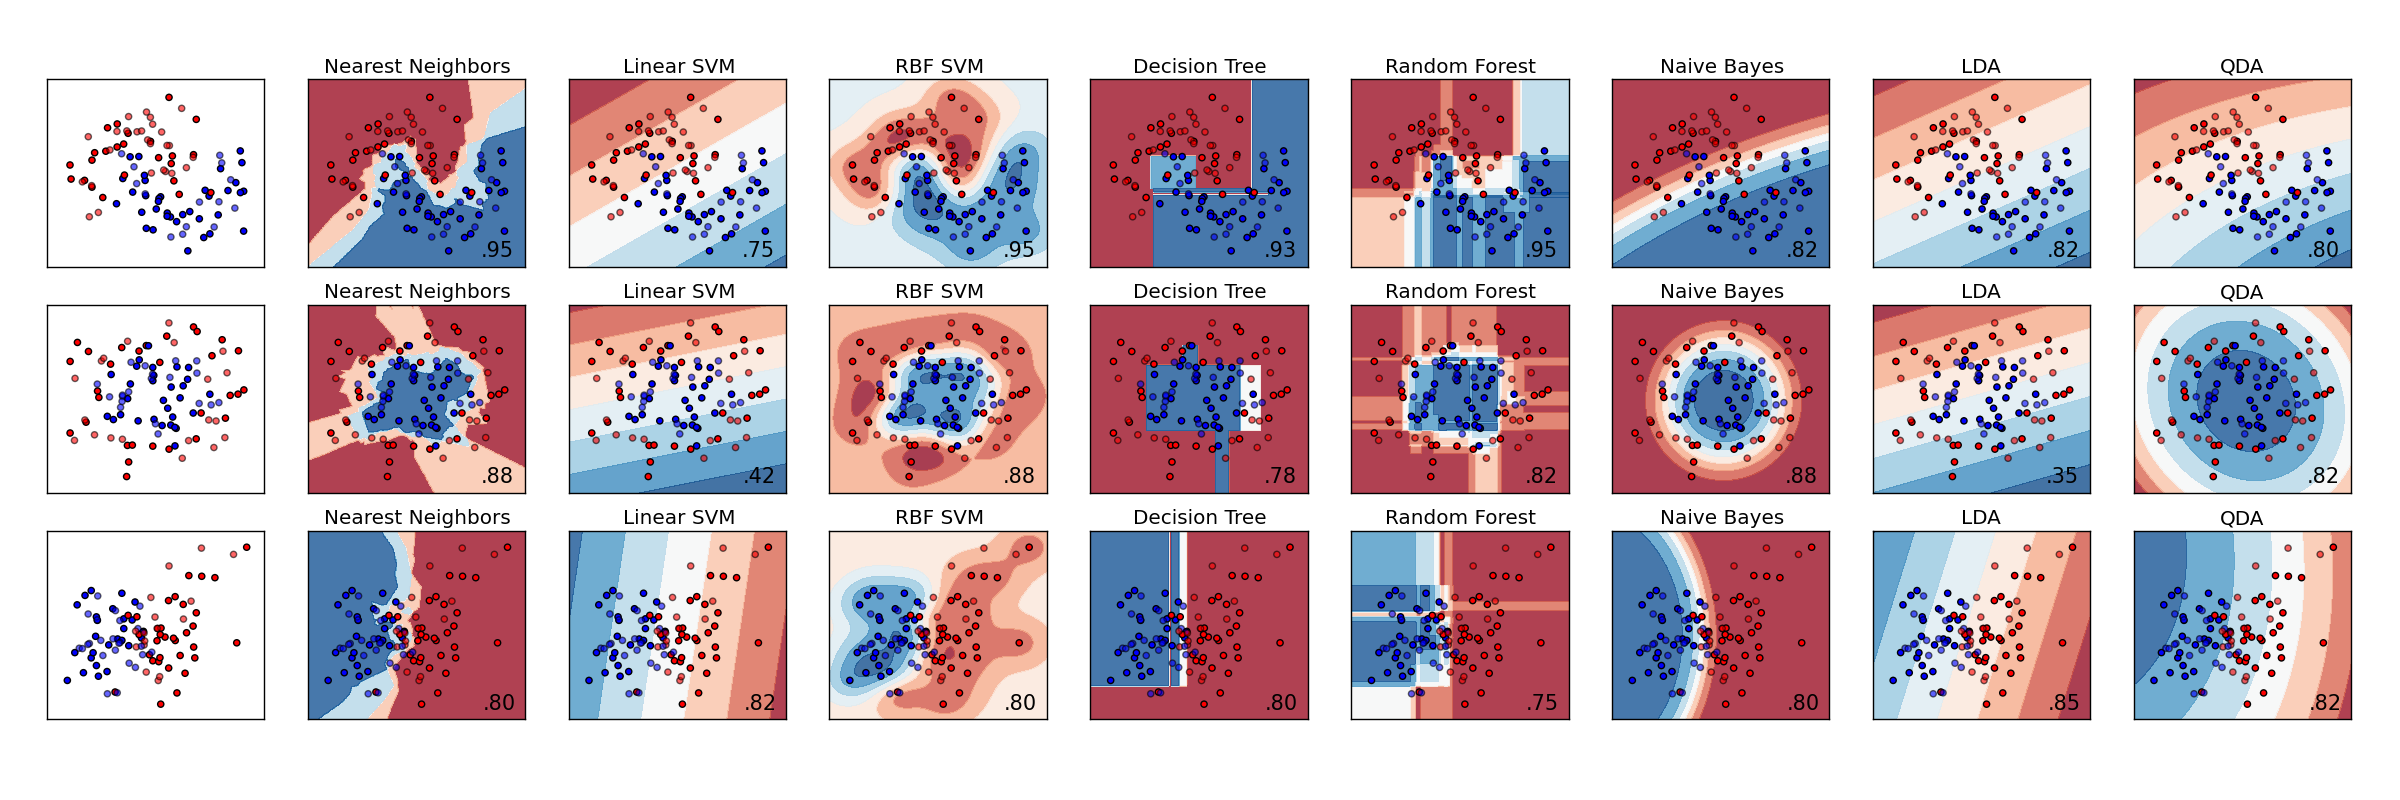
\includegraphics[width=1.1\textwidth]{figs/classifiers}
\end{figure}
\end{center} 
\
\end{frame}

% section Classfication (end)


%----------------------------FRAME------------------------------------
\begin{frame}[fragile]\frametitle{k-nearest neighbours }
%-------------------------------CODE
\begin{minted}[bgcolor=mybg,frame=lines,mathescape]{python}
>>> from sklearn import neighbors
>>> knn = neighbors.KNeighborsClassifier(7)
>>> knn.fit(T, y)
KNeighborsClassifier(algorithm='auto', leaf_size=30, n_neighbors=7, p=2,
           warn_on_equidistant=True, weights='uniform')
>>> knn.predict([[0.1, 0.2]])
array([1])
>>> yPred = knn.predict(T)
>>> (yPred==y).mean()
0.97999999999999998
\end{minted}

%-------------------------------END CODE
\end{frame}

%----------------------------FRAME------------------------------------
\begin{frame}[fragile]\frametitle{Support Vector Classification}
%-------------------------------CODE
\begin{minted}[bgcolor=mybg,frame=lines,mathescape]{python}
>>> from sklearn import svm
>>> C,gamma = 1,0.7
>>> svcg = svm.SVC(kernel='rbf', gamma=gamma, C=C).fit(T, y)
>>> svcg.predict([-.7,7])
array([ 2.])
>>> yPred = svcg.predict(T)
>>> (yPred==y).mean()
0.95333333333333337
\end{minted}

%-------------------------------END CODE
\end{frame}

\subsection{Metrics} % (fold)
\label{ssub:Metrics}
%----------------------------FRAME------------------------------------
\begin{frame}[fragile]\frametitle{sklearn.metrics}
\begin{block}{sklearn.metrics}
\begin{description}
    \item[roc\_curve]  Compute Receiver operating characteristic (ROC).
    \item[precision\_recall\_curve] Compute precision-recall pairs for different probability thresholds.
    \item[accuracy\_score] Accuracy classification score.
    \item[confusion\_matrix] Confusion matrix. 
    \item[matthews\_corrcoef] Matthews Correlation coefficient
    \item[classification\_report] Build a text report showing the main classification metrics.
 \end{description}
\end{block}

\end{frame}

%----------------------------FRAME------------------------------------
\begin{frame}[fragile]\frametitle{sklearn.metrics}
%-------------------------------CODE
\begin{minted}[bgcolor=mybg,frame=lines,mathescape]{python}
>>> from sklearn import metrics
>>> metrics.recall_score(yPred,y)
0.95333333333333337
>>> metrics.confusion_matrix(yPred,y)
array([[50,  0,  0],
       [ 0, 47,  4],
       [ 0,  3, 46]])
\end{minted}

\begin{minted} [bgcolor=mybg,frame=lines,bgcolor=mybg,frame=lines,bgcolor=mybg,frame=lines,mathescape]{python}
metrics.classification_report(yPred,y)
             precision    recall  f1-score   support
          0       1.00      1.00      1.00        50
          1       0.94      0.92      0.93        51
          2       0.92      0.94      0.93        49
navg / total       0.95      0.95      0.95       150
\end{minted}

%-------------------------------END CODE

\end{frame}

% subsubsection Metrics (end)

\subsection{Cross Validation} % (fold)
\label{ssub:Cross Validation}

%----------------------------FRAME------------------------------------
\begin{frame}[fragile]\frametitle{Cross-validation}
\begin{center}
   \centering
        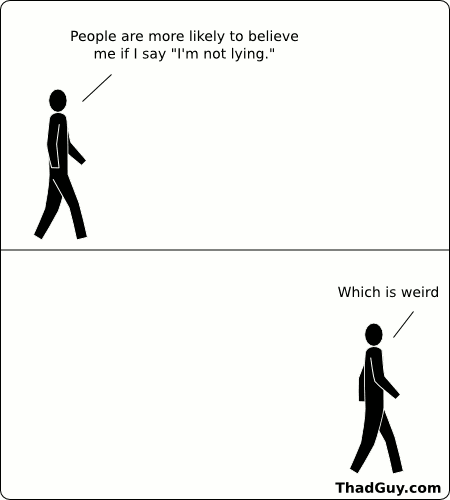
\includegraphics[width=0.5\textwidth]{figs/imnotlying}
\end{center} 

\end{frame}


\begin{frame}
  \frametitle{Validity and Over-Fitting}
  \begin{block}{}
    In multivariate predictive models, \textcolor{blue}{over-fitting} occurs when a
    large number of predictor variables is fit to a small N of
    subjects.  A model may ``fit'' well or perfectly, even if no real
    relationship.  Simon, JNCI 2003
  \end{block}
  \pause \begin{block}{Direct Consequence of Over-fitting}
    Model performance results are not reproducible in a
    \textcolor{blue}{new} set of data. 
  \end{block}
\end{frame}

\begin{frame}
  \frametitle{Over-Fitting}
  \begin{center}
    \centering 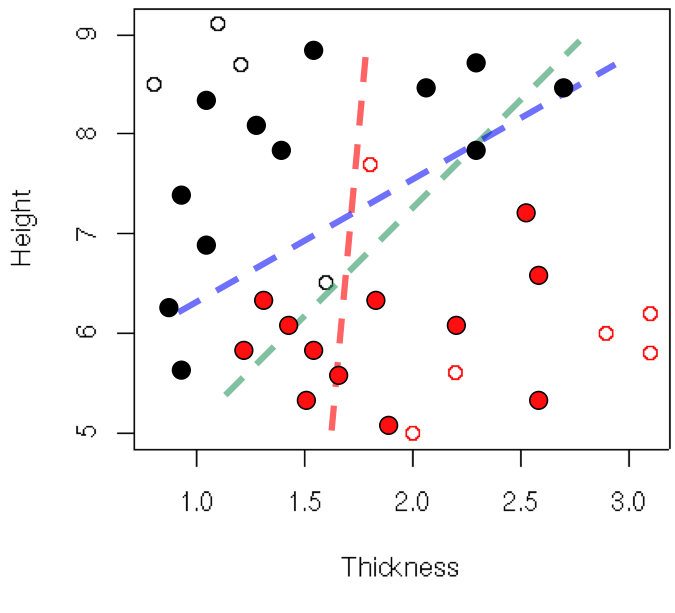
\includegraphics[width=0.6\textwidth]{figs/2vars}
  \end{center}
\end{frame}



\begin{frame}
  \frametitle{Validation Schemes}
  \begin{center}
    \centering 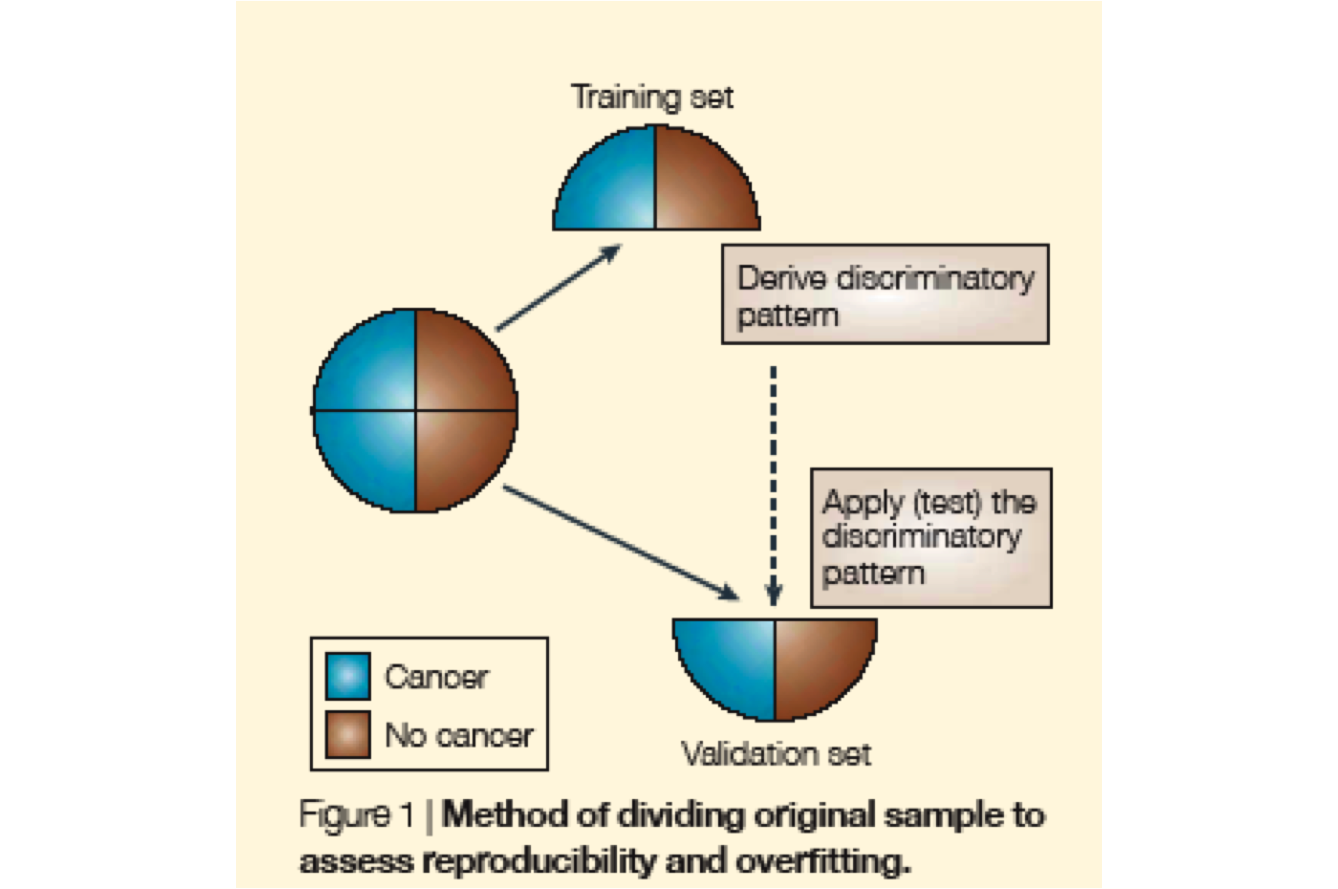
\includegraphics[width=0.7\textwidth]{figs/crossval}
  \end{center}
\tiny{Ransohoff.  Nat Rev Cancer 2004 }
\end{frame}

%----------------------------FRAME------------------------------------
\begin{frame}[fragile]\frametitle{Cross Validation}
\begin{block}{sklearn.cross\_validation.train\_test\_split}
Split arrays or matrices into random train and test subsets.
\end{block}
\small
%-------------------------------CODE
\begin{minted}[bgcolor=mybg,frame=lines,mathescape]{python}
>>> from sklearn import cross_validation
>>> xTrain, xVal, yTrain, yVal = cross_validation.train_test_split(
...     X, y, test_size=0.4)
... 
>>> xTrain.shape,xVal.shape
((90, 4), (60, 4))
\end{minted}

\pause 
%-------------------------------CODE
\begin{minted}[bgcolor=mybg,frame=lines,mathescape]{python}
>>> from sklearn import neighbors
>>> knn = neighbors.KNeighborsClassifier(7).fit(xTrain, yTrain)
>>> yPredVal = knn.predict(xVal)
>>> (yPredVal==yVal).mean()
0.93333333333333335
\end{minted}

%-------------------------------END CODE
%-------------------------------END CODE
\end{frame}

%----------------------------FRAME------------------------------------
\begin{frame}[fragile]\frametitle{Cross-validation metrics}
Can we compute some statistics on the performance of the classifiers? \verb|cross_val_score| exists! 
%-------------------------------CODE
\begin{minted}[bgcolor=mybg,frame=lines,mathescape]{python}
>>> knn = neighbors.KNeighborsClassifier(1)
>>> recalls = cross_validation.cross_val_score(
...     knn, X, y, cv = 6)
... 
>>> recalls
array([ 0.92,  0.96,  0.96,  1.  ,  0.96,  0.96])
>>> recalls.mean()
0.95999999999999996
>>> recalls.std()
0.023094010767585018
\end{minted}

%-------------------------------END CODE

\end{frame}

%----------------------------FRAME------------------------------------
\begin{frame}[fragile]\frametitle{Leave one out}
\begin{block}{LOO}
Each training set is constructed  by taking all samples except sample $k$ and the model validates over $k$. Then just iterate through $k$. 
\end{block}
%-------------------------------CODE
\begin{minted}[bgcolor=mybg,frame=lines,mathescape]{python}
>>> from sklearn.cross_validation import LeaveOneOut
>>> from sklearn import svm
>>> loo = LeaveOneOut(y.size)
>>> cl = svm.SVC(kernel='linear', C=1)
>>> recalls = [(y[indVal] == cl.fit(X[indTrain,:],y[indTrain]).\
...         predict(X[indVal,:])).mean() \
...             for indTrain, indVal in loo]
... 
>>> len(recalls)
150
>>> recalls[:5]
[1.0, 1.0, 1.0, 1.0, 1.0]
\end{minted}

%-------------------------------END CODE
\end{frame}

% subsubsection Cross Validation (end)

%----------------------------FRAME------------------------------------
\begin{frame}[fragile]\frametitle{k-nearest neighbours vs. SVC Challenge}
\begin{block}{Challenge}
\begin{enumerate}
    \item Get all variables from Iris dataset.
    \item Compute a 2D-PCA model of the Iris dataset.
    \item Compute and plot the decision boundaries for a k-NN and SVC classifier of your choice.   
 
\end{enumerate}
\end{block}

Hint: use np.mesgrid() 
\end{frame}




% section Clustering (end)

% section scikit-learn (end)


\section{A Practical Introduction to Scikit-learn} % (fold)
\label{sec:A Practical Introduction to Scikit-learn}





% section A Practical Introduction to Scikit-learn (end)
\begin{frame}
	\setbeamercovered{dynamic}
	\frametitle{  An Eigenfaces Session with python }
This session aims to demonstrate the use of scikit in python using an eigenfaces exercise. 
\begin{enumerate}
    \item First will construct a class for storing the information of the chamber of representatives. 
    \item Later we will import the image dataset, 
    \item compute some descriptive statistics, 
    \item perform an analysis of principal components,
    \item clustering analysis and finally, 
    \item will use a non-linear classifier to assess the gender from just the image of the representative.

\end{enumerate}
\end{frame}



\subsection{Data Description}


\begin{frame}
  \frametitle{www.congreso.es}
  \begin{itemize}
  \item Public database (members of the Chamber of Representatives)
  \item Small  \emph{python} script extracted picture and info for
    each representative
  \end{itemize}
  
 \only<1>{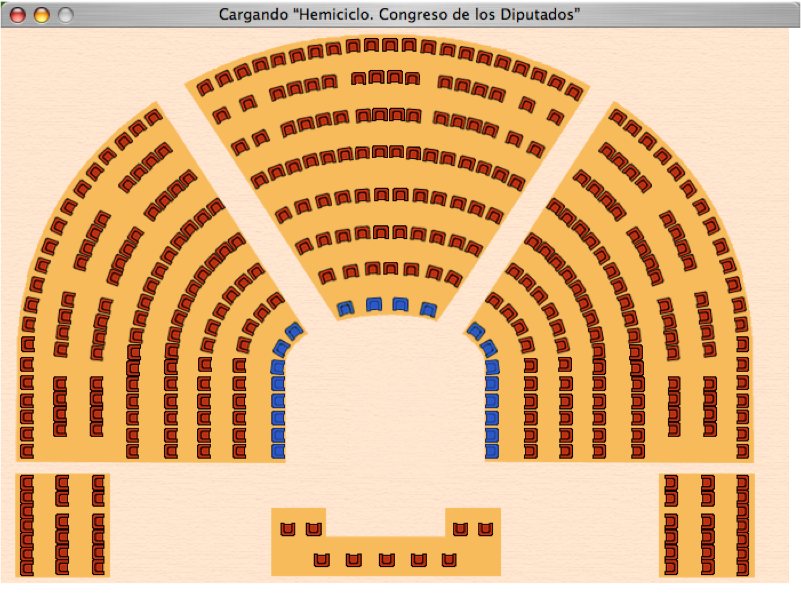
\includegraphics[width=0.75\textwidth]{figs/congreso}}
 \only<2>{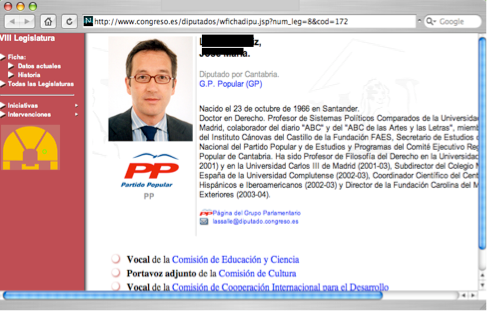
\includegraphics[width=0.8\textwidth]{figs/dipulassalle}}
 \only<3>{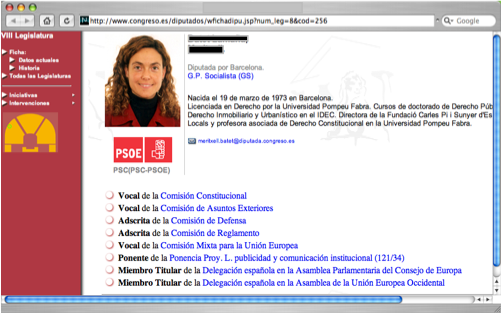
\includegraphics[width=0.8\textwidth]{figs/diputxell}}
 \only<4>{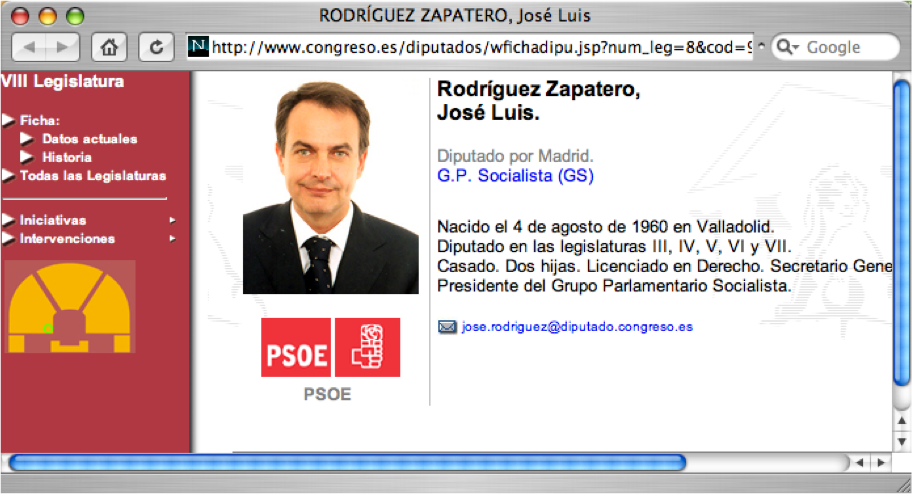
\includegraphics[width=0.8\textwidth]{figs/dipujose}}
 \only<5>{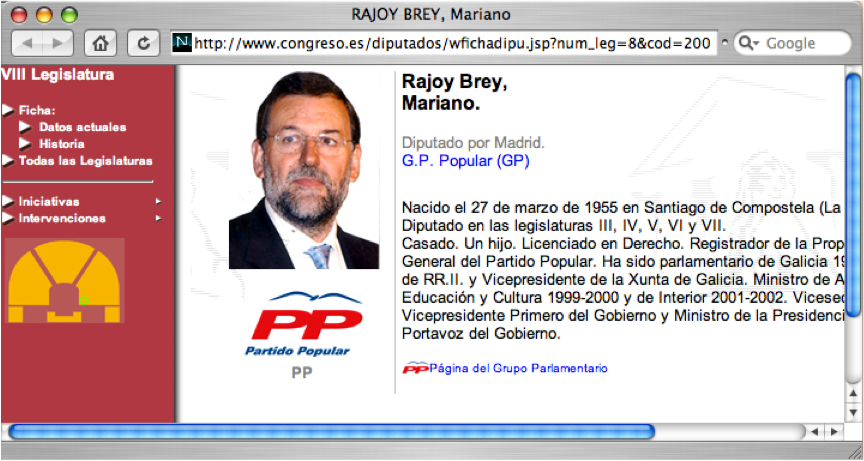
\includegraphics[width=0.8\textwidth]{figs/dipurajoy}}

\end{frame}




\begin{frame}
  \frametitle{www.congreso.es}
  \begin{itemize}
  \item Images imported and converted to B/W
  \item 350 members, $86 \times 85 =7310$ pixels
  \end{itemize}
  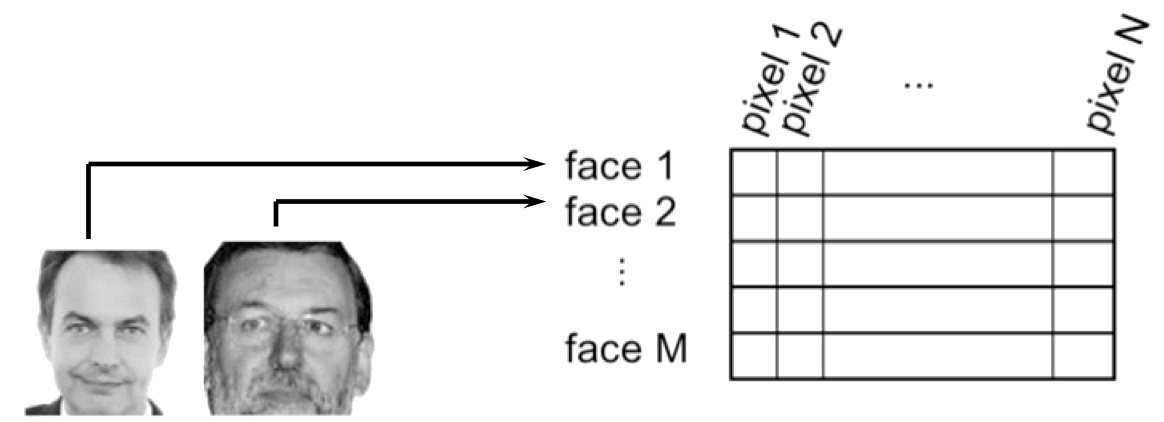
\includegraphics[width=0.85\textwidth]{figs/features}  
\end{frame}

\subsection{Importing Data}


\begin{frame}
	\setbeamercovered{dynamic}
	\frametitle{  Preparing to import the data}
	We will need to define some classes to prepare the image readout. A nice way of doing this is defining a \emph{Diputado} class, followed by a \emph{Parlamento}	
	A \emph{Diputado}  has a Name, Surnames, ID, Picture, Gender and Political Affiliation.
\end{frame}

\begin{frame}[fragile,allowframebreaks]
	\setbeamercovered{dynamic}
	\frametitle{ A Diputado class definition}
\small
\begin{columns}
\column{0.5\textwidth}
\begin{minted} [bgcolor=mybg,frame=lines,bgcolor=mybg,frame=lines,bgcolor=mybg,frame=lines,mathescape]{python}
class Diputado(object):
    def __init__(self,ind,fileRoot="./"):
        self.name=""
        self.surname=""
        self.ind=ind
        self.picfile=""        
        self.party=""
        self.gender=""
        self.fileRoot=fileRoot
        self.ext='c.jpg'
    def setName(self,name):
        self.name=name
    def setSurname(self,surname):
        self.surname=surname
    def setParty(self,party):
        self.party=party
    def setGender(self,gender):
        self.gender=gender
\end{minted}
\column{0.5\textwidth}
\begin{minted} [bgcolor=mybg,frame=lines,bgcolor=mybg,frame=lines,bgcolor=mybg,frame=lines,mathescape]{python}
    def getName(self):
        return self.name
    def getSurname(self): 
        return self.surname
    def getInd(self):
        return self.ind
    def getPicfile(self):
        return self.fileRoot + str(self.ind) + self.ext
    def getParty(self):
        return self.party
    def getGender(self):
        return self.gender
\end{minted}
\end{columns}
\end{frame} 




%----------------------------FRAME------------------------------------
\begin{frame}[fragile]\frametitle{Parlament class}
%-------------------------------CODE
\tiny
\begin{minted} [bgcolor=mybg,frame=lines,bgcolor=mybg,frame=lines,bgcolor=mybg,frame=lines,mathescape]{python}
class Parlament(object):
    def __init__(self):
        self.elements=[]
        self.inds=[]
        self.ndips=0
    def add(self, diputado):
        self.elements.append(diputado)
        self.inds.append(diputado.getInd())
        self.ndips +=1
    def getInds(self):
        return [self.elements[i].getInd() for i in range(self.ndips)]
    def len(self):
        return len(self.elements)
    def __getitem__(self, key):
        if isinstance(key, slice):
            indices = key.indices(self.ndips)
            return [self[ii] for ii in xrange(*key.indices(self.len()))] 
        else:
            return self.elements[key]
    def getName(self,key):
        return self.elements[key].getName()
\end{minted}


%-------------------------------END CODE
\end{frame}
%----------------------------FRAME------------------------------------
\begin{frame}[fragile]\frametitle{Importing data images}
\begin{minted} [bgcolor=mybg,frame=lines,bgcolor=mybg,frame=lines,bgcolor=mybg,frame=lines,mathescape]{python}
import csv
with open('db/index.csv','rb') as csvfile:
    r = csv.reader(csvfile, delimiter=';')
    r.next()
    p = Parlament()
    for row in r:
        n = Diputado(int(row[0]),"db/db/")
        n.setName(row[1].strip())
        n.setSurname(row[2].strip())
        n.setGender(row[3].strip())
        n.setParty(row[4].strip())
        p.add(n)

\end{minted}
%-------------------------------CODE

%-dd-----------------------dd-------END CODE
\end{frame}

%----------------------------FRAME------------------------------------
\begin{frame}[fragile]\frametitle{Let's see what we have}
%-------------------------------CODE
\begin{minted}[bgcolor=mybg,frame=lines,mathescape]{python}
from scipy import ndimage,misc
from numpy import shape,prod,unique,sqrt
import matplotlib.pyplot as pl
I = ndimage.imread(p[1].getPicfile())
pl.imshow(I)
shape(I)
'|'.join([p[1].getName(), p[1].getSurname(), p[1].getGender()])
\end{minted}

%-------------------------------END CODE
\end{frame}
%----------------------------FRAME------------------------------------
\begin{frame}[fragile]\frametitle{Let's see what we have}
\begin{columns}
    \column{0.7\columnwidth}
%-------------------------------CODE
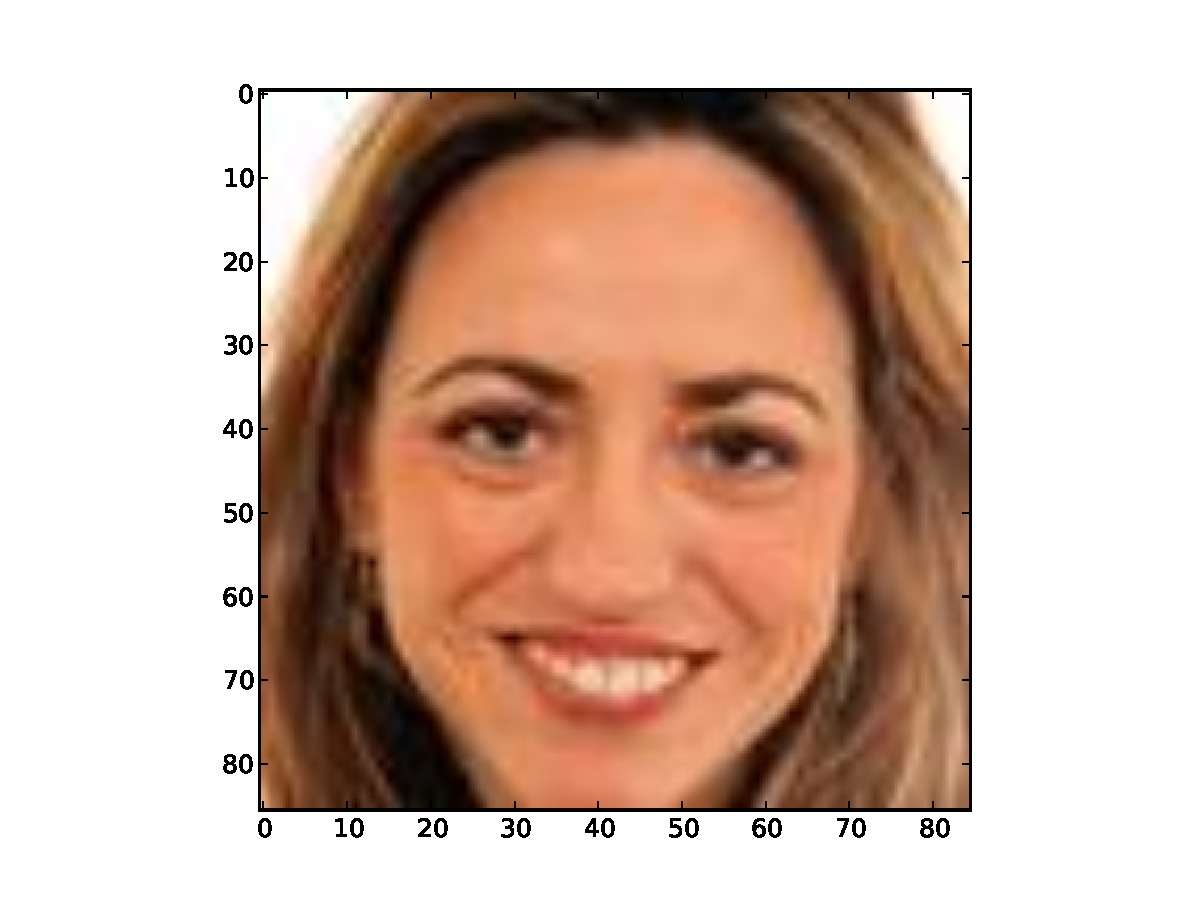
\includegraphics[width=\textwidth]{plwfigis/CursP_4_figure20}

%-------------------------------END CODE
\end{columns}

\end{frame}

%----------------------------FRAME------------------------------------
\begin{frame}[fragile]\frametitle{Converting to gray}
%-------------------------------CODE
\begin{minted}[bgcolor=mybg,frame=lines,mathescape]{python}
I = ndimage.imread(p[1].getPicfile(), flatten=1)
img=pl.imshow(I)
img.set_cmap('gray')
Is=shape(I)
Is
\end{minted}

%-------------------------------END CODE
\begin{columns}
    \column{0.7\columnwidth}
%-------------------------------CODE
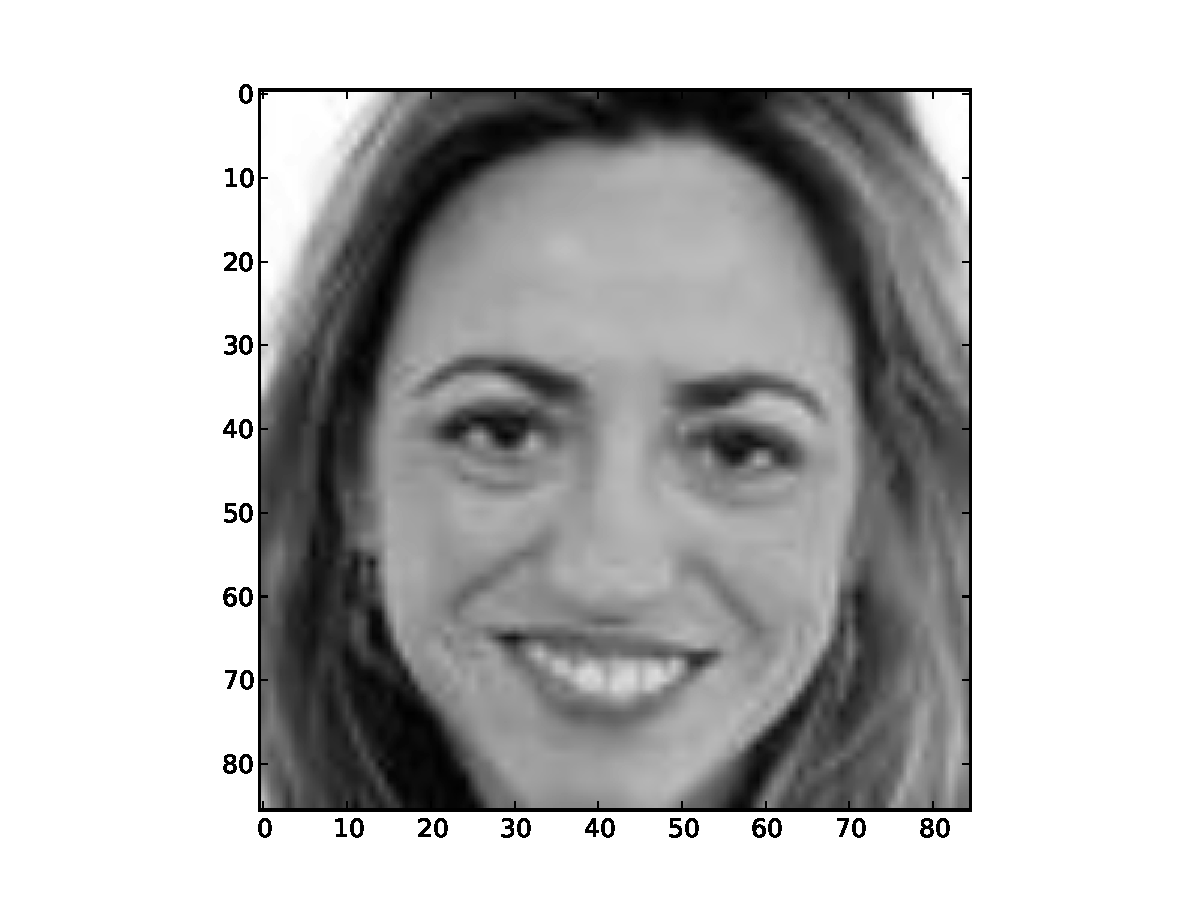
\includegraphics[width=\textwidth]{plwfigis/CursP_4_figure22}

%-------------------------------END CODE
\end{columns}
\end{frame}

%----------------------------FRAME------------------------------------
\begin{frame}[fragile]\frametitle{And everything is a Signal...}
%-------------------------------CODE

\begin{columns}
    \column{0.8\columnwidth}

\begin{minted}[bgcolor=mybg,frame=lines,mathescape]{python}
Iv = np.reshape(I,prod(Is))
pl.plot(Iv)
\end{minted}
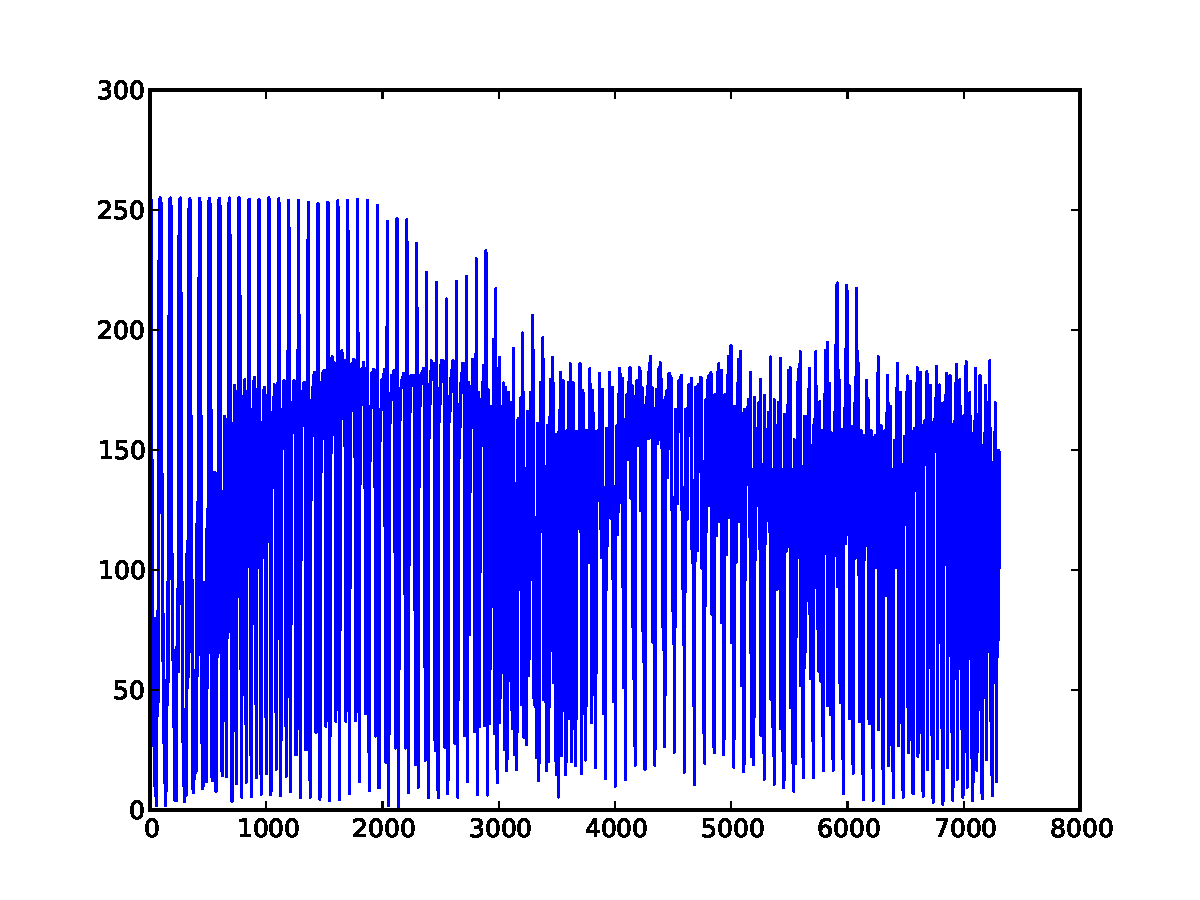
\includegraphics[width=\textwidth]{plwfigis/CursP_4_figure23}

\end{columns}

%-------------------------------END CODE
\end{frame}
%----------------------------FRAME------------------------------------
\begin{frame}[fragile]\frametitle{Construct the final dataset}
%-------------------------------CODE
\begin{minted}[bgcolor=mybg,frame=lines,mathescape]{python}
>>> X=np.array([ np.reshape(ndimage.imread(p[i].getPicfile(), \
...                 flatten=1), prod(Is)) \
...              for i in range(0,p.len())])
... 
>>> shape(X)
(348, 7310)
>>> Yg=np.array([ p[i].getGender() \
...     for i in range(0,p.len())])
... 
>>> Yp=np.array([ p[i].getParty() \
...     for i in range(0,p.len())])
... 
>>> Yp[0:5],Yg[0:5],shape(X)
(array(['GS', 'GS', 'GC-CiU', 'GP', 'GP'], 
      dtype='|S10'), array(['H', 'M', 'H', 'H', 'H'], 
      dtype='|S1'), (348, 7310))
\end{minted}

%-------------------------------END CODE
\end{frame}



\subsection{Unsupervised Analysis}
\subsubsection{Principal Component Analysis}
%----------------------------FRAME------------------------------------
\begin{frame}[fragile]\frametitle{Principal Component Analysis}
Now begins the interesting part. Let's try a PCA projection.
%-------------------------------CODE
\begin{minted}[bgcolor=mybg,frame=lines,mathescape]{python}
>>> from sklearn.decomposition import PCA
>>> from sklearn import preprocessing
>>> sX = preprocessing.scale(X)
>>> ncomp=5
>>> mod=PCA(n_components=ncomp)
>>> mod.fit(sX)
PCA(copy=True, n_components=5, whiten=False)
>>> ev = mod.explained_variance_ratio_
>>> print(ev)
[ 0.21537468  0.08870527  0.07254977  0.05253376  0.04564393]
\end{minted}

%-------------------------------END CODE
\end{frame}
%----------------------------FRAME------------------------------------
\begin{frame}[fragile]\frametitle{Principal Component Analysis}
The projection over the embedding.
%-------------------------------CODE
\begin{minted}[bgcolor=mybg,frame=lines,mathescape]{python}
>>> Xpca = mod.transform(sX)
>>> Xpca[0:3,:]
array([[-35.67224884,  -2.5693078 ,  13.0386591 ,   7.5424757 ,
        -10.67783451],
       [ 55.11857986, -19.39882469, -26.91612053, -21.87864685,
         -6.68953943],
       [-36.31109619,  -0.79103142,  -9.56684589, -20.49104309,
         -3.42452836]], dtype=float32)
\end{minted}

%-------------------------------END CODE
\end{frame}
%----------------------------FRAME------------------------------------
\begin{frame}[fragile]\frametitle{Eigendiputados}
The principal components can be interpreted.
%-------------------------------CODE
\small
\begin{minted}[bgcolor=mybg,frame=lines,mathescape]{python}
eigendips = mod.components_.reshape((ncomp, Is[0], Is[1]))

pl.figure(figsize=(9 ,3))

pl.subplot(131)
pl.imshow(eigendips[0], cmap=pl.cm.gray)
pl.axis('off')

pl.subplot(132)
pl.imshow(eigendips[1], cmap=pl.cm.gray)
pl.axis('off')

pl.subplot(133)
pl.imshow(-eigendips[2], cmap=pl.cm.gray)
pl.axis('off')

pl.subplots_adjust(wspace=0.01, hspace=0.01, top=1, bottom=0, left=0, right=1)
\end{minted}

%-------------------------------END CODE
\end{frame}
%----------------------------FRAME------------------------------------
\begin{frame}[fragile]\frametitle{Eigendiputados}
%-------------------------------CODE
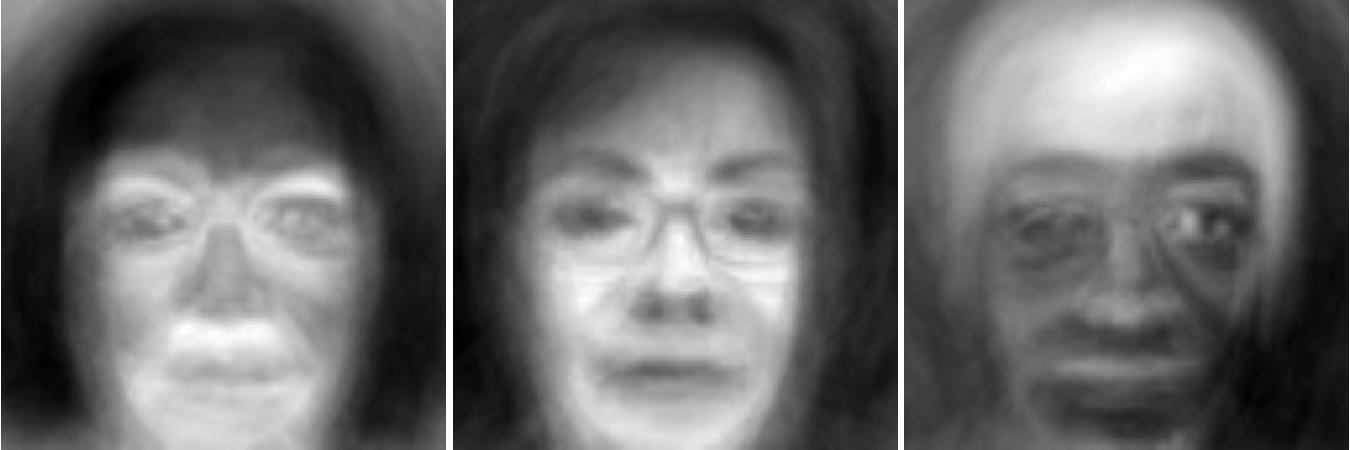
\includegraphics[width=\textwidth]{plwfigis/CursP_4_figure28}

%-------------------------------END CODE
\end{frame}

%----------------------------FRAME------------------------------------
\begin{frame}[fragile]\frametitle{Score plots}
%-------------------------------CODE
\begin{minted}[bgcolor=mybg,frame=lines,mathescape]{python}
colors=['blue','red']
clut = dict(zip(['M','H'],['red','blue']))
""" for one shot plot cols=[ clut[i] for i in Yg]"""

pl.scatter(Xpca[np.where(Yg=='H'),0],\
    Xpca[np.where(Yg=='H'),1],c='red')
pl.scatter(Xpca[np.where(Yg=='M'),0],\
    Xpca[np.where(Yg=='M'),1],c='blue')
pl.legend(('M','H'))
pl.xlabel('1PC ('+ "%s" % float( "%2.1g" % (100*ev[0])) +"%)")
pl.ylabel('2PC ('+ "%s" % float( "%2.1g" % (100*ev[1])) +"%)")
\end{minted}

%-------------------------------END CODE
\end{frame}
%----------------------------FRAME------------------------------------
\begin{frame}[fragile]\frametitle{Score plots}
%-------------------------------CODE
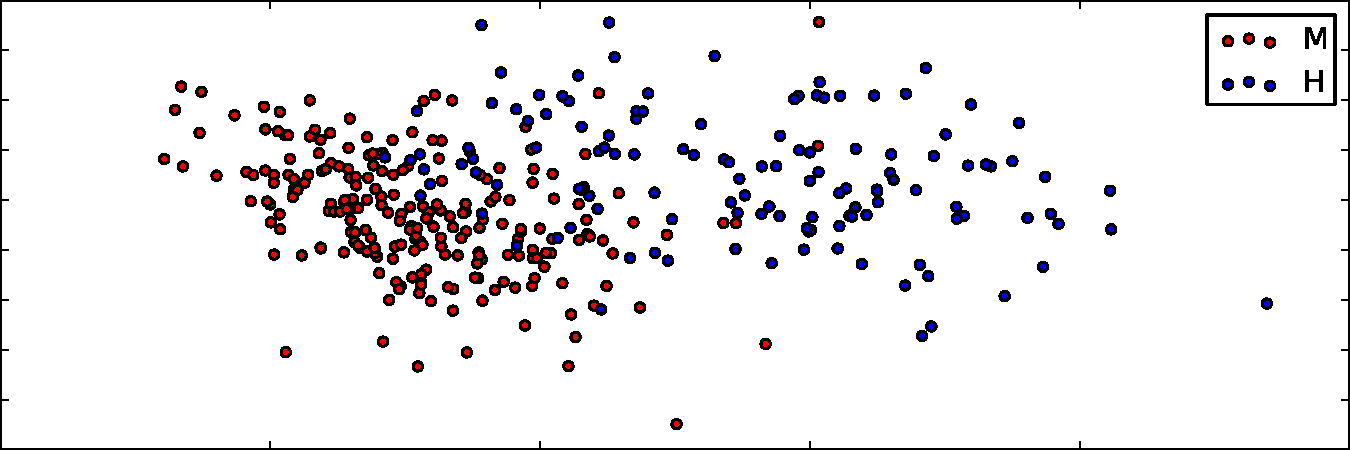
\includegraphics[width=\textwidth]{plwfigis/CursP_4_figure30}

%-------------------------------END CODE
\end{frame}

\subsubsection{Clustering}
%----------------------------FRAME------------------------------------
\begin{frame}[fragile]\frametitle{k-means}
With the data already imported, it's easy to group similar pictures with a clustering algorithm.
%-------------------------------CODE
\begin{minted}[bgcolor=mybg,frame=lines,mathescape]{python}
>>> from sklearn import cluster
>>> 
>>> k_means =  cluster.KMeans(k=8,n_init=10)
>>> k_means.fit(Xpca)
KMeans(copy_x=True, init='k-means++', k=8, max_iter=300, n_init=10, n_jobs=1,
    precompute_distances=True,
    random_state=<mtrand.RandomState object at 0x7f6d01af51b0>, tol=0.0001,
    verbose=0)
>>> 
>>> pl.scatter(Xpca[:,0],Xpca[:,1],c=k_means.labels_.astype(np.float))
<matplotlib.collections.PathCollection object at 0x3afcd90>
\end{minted}

%-------------------------------END CODE
\end{frame}
%----------------------------FRAME------------------------------------
\begin{frame}[fragile]\frametitle{k-means}
%-------------------------------CODE
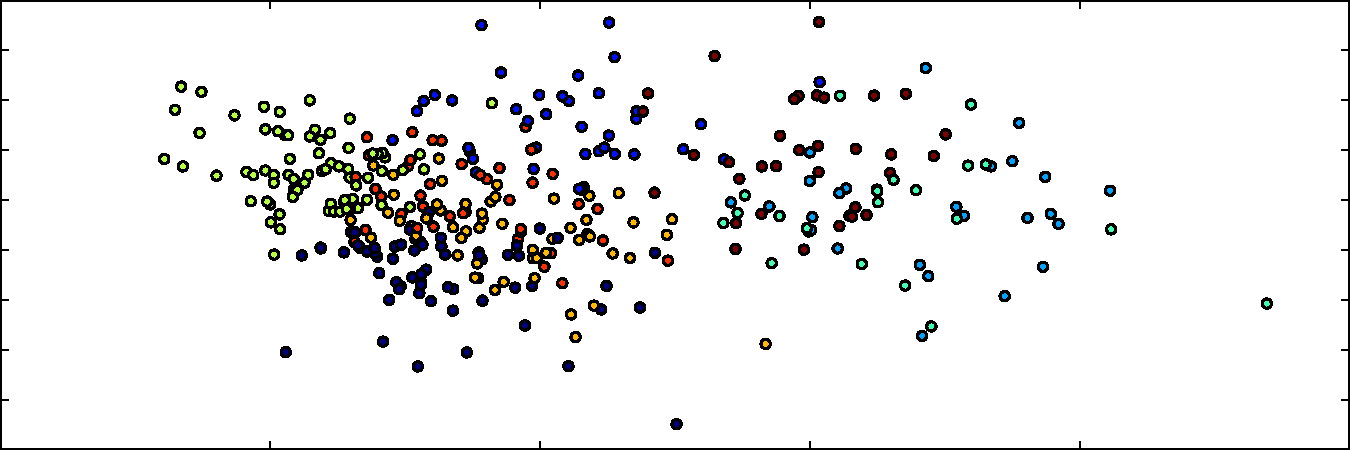
\includegraphics[width=\textwidth]{plwfigis/CursP_4_figure32}

%-------------------------------END CODE
\end{frame}

%----------------------------FRAME------------------------------------
\begin{frame}[fragile]\frametitle{k-means}
\begin{block}{}
We can plot the samples that have been grouped within the same cluster. For doing so we have to reshape the vectors corresponding to each sample matching the original images. This is extremely easy to do in python!
\end{block}
\begin{minted} [bgcolor=mybg,frame=lines,bgcolor=mybg,frame=lines,bgcolor=mybg,frame=lines,mathescape]{python}
def plotg(g):
    indg = np.where(k_means.labels_ == g)
    nx = int(sqrt(shape(indg)[1]))+1
    ny = nx+1
    f = pl.figure()

    for e,i in enumerate(indg[0]):
        f.add_subplot(ny,nx,e)
        pl.imshow(X[i,:].reshape(Is), cmap=pl.cm.gray)
        pl.axis('off')
      
\end{minted}

%-------------------------------CODE

%-------------------------------END CODE
\end{frame}
%----------------------------FRAME------------------------------------
\begin{frame}[fragile]\frametitle{k-means groups}
%-------------------------------CODE
\small 
\begin{minted}[bgcolor=mybg,frame=lines,mathescape]{python}
>>> print(unique(k_means.labels_))
[0 1 2 3 4 5 6 7]
>>> plotg(5), plotg(0)
(None, None)
\end{minted}
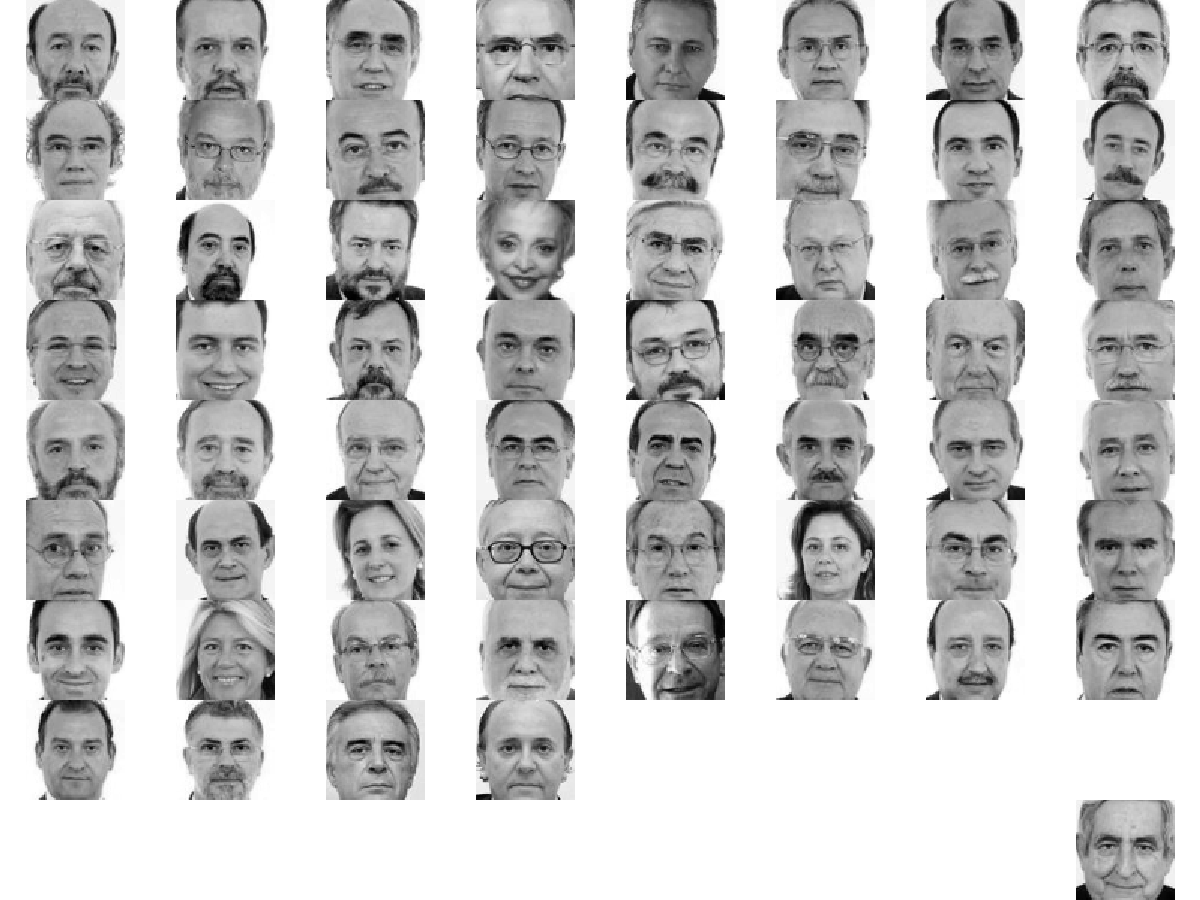
\includegraphics[width=\textwidth]{plwfigis/CursP_4_figure33}

%-------------------------------END CODE
\end{frame}


\subsection{Supervised Analysis}
\subsubsection{k-Nearest Neighbours}

%----------------------------FRAME------------------------------------
\begin{frame}[fragile]\frametitle{Supervised Analysis}
\begin{block}{}
Next, we will build two classifiers and will try to asses gender just from the feature vector (pixel intensities). We will test k-nn classifier and compare it with a Support Vector Classifier, trained with a grid search. We will also show how to use a cross-validation scheme provided by sklearn scipy toolkit.
\end{block}

\end{frame}
%----------------------------FRAME------------------------------------
\begin{frame}[fragile]\frametitle{Supervised analysis}
%-------------------------------CODE
\begin{minted}[bgcolor=mybg,frame=lines,mathescape]{python}
>>> nYg = np.array([ int(y=='H') for y in Yg])
>>> print nYg[0:5]
[1 0 1 1 1]
\end{minted}

%-------------------------------END CODE
\end{frame}
%----------------------------FRAME------------------------------------
\begin{frame}[fragile]\frametitle{k-Neighbors Classifier}
%-------------------------------CODE
\begin{minted}[bgcolor=mybg,frame=lines,mathescape]{python}
from sklearn.neighbors import KNeighborsClassifier
from sklearn import cross_validation
k_fold = cross_validation.KFold(n=p.len(), k=3, indices=True)
scores = list()
for train_indices, test_indices in k_fold:
    Xtrain = X[train_indices,:]
    Ytrain = nYg[train_indices]
    Xval = X[test_indices,:]
    Yval = nYg[test_indices]
    knn = KNeighborsClassifier()
    knn.fit(Xtrain,Ytrain)
    scores.append(knn.score(Xval,Yval))
\end{minted}

%-------------------------------END CODE
\end{frame}
%----------------------------FRAME------------------------------------
\begin{frame}[fragile]\frametitle{}
%-------------------------------CODE
\small
\begin{minted}[bgcolor=mybg,frame=lines,mathescape]{python}
>>> [knn.fit(X[train,:], nYg[train]).score(X[test,:], nYg[test]) 
...     for train, test in k_fold]
... 
[0.81896551724137934, 0.89655172413793105, 0.90517241379310343]
\end{minted}

%-------------------------------END CODE
\end{frame}


\subsubsection{Support Vector Classification}
%----------------------------FRAME------------------------------------
\begin{frame}[fragile]\frametitle{Support Vector Classifier}
%-------------------------------CODE
\small
\begin{minted}[bgcolor=mybg,frame=lines,mathescape]{python}
>>> from sklearn import svm
>>> svc = svm.SVC(C=1, kernel='linear')
>>> [svc.fit(X[train,:], nYg[train]).score(X[test,:], nYg[test]) 
...     for train, test in k_fold]
... 
[0.84482758620689657, 0.89655172413793105, 0.89655172413793105]
\end{minted}

%-------------------------------END CODE
\end{frame}

%----------------------------FRAME------------------------------------
\begin{frame}[fragile]\frametitle{Support Vector Classifier}
In fact, we should cross-validate with some balance on the class folds.
%-------------------------------CODE
\begin{minted}[bgcolor=mybg,frame=lines,mathescape]{python}
k_fold_class_balanced = \
    cross_validation.StratifiedKFold(nYg,k=5)

svc = svm.SVC(C=1, kernel='linear')
[svc.fit(X[train,:], nYg[train]).score(X[test,:], nYg[test]) 
    for train, test in k_fold_class_balanced]
\end{minted}

%-------------------------------END CODE
\end{frame}

%----------------------------FRAME------------------------------------
\begin{frame}[fragile]\frametitle{SCV tunning}
%-------------------------------CODE
\small 
\begin{minted}[bgcolor=mybg,frame=lines,mathescape]{python}
>>> from sklearn.grid_search import GridSearchCV
>>> gammas = np.logspace(-6, -1, 5)
>>> clf = GridSearchCV(estimator=svc, param_grid=dict(gamma=gammas), n_jobs=-1)
>>> clf.fit(X[train,:], nYg[train]) 
GridSearchCV(cv=None,
       estimator=SVC(C=1, cache_size=200, class_weight=None, coef0=0.0, degree=3, gamma=0.0,
  kernel='linear', probability=False, shrinking=True, tol=0.001,
  verbose=False),
       fit_params={}, iid=True, loss_func=None, n_jobs=-1,
       param_grid={'gamma': array([  1.00000e-06,   1.77828e-05,   3.16228e-04,   5.62341e-03,
         1.00000e-01])},
       pre_dispatch='2*n_jobs', refit=True, score_func=None, verbose=0)
>>> print clf.best_score_
0.888888888889
>>> print clf.best_estimator_.gamma
1e-06
>>> print clf.score(X[test,:], nYg[test])
0.898550724638
\end{minted}

%-------------------------------END CODE
\end{frame}
%----------------------------FRAME------------------------------------
\begin{frame}[fragile]\frametitle{Performance}
%-------------------------------CODE
\begin{minted}[bgcolor=mybg,frame=lines,mathescape]{python}
>>> from sklearn.metrics import classification_report
>>> ypred = clf.predict(X[test,:])
>>> ytest = nYg[test]
>>> ygtest = Yg[test]
>>> print classification_report(ytest, ypred, target_names=['H','M'])
             precision    recall  f1-score   support

          H       0.91      0.80      0.85        25
          M       0.89      0.95      0.92        44

avg / total       0.90      0.90      0.90        69

\end{minted}

%-------------------------------END CODE
\end{frame}

%----------------------------FRAME------------------------------------
\begin{frame}[fragile]\frametitle{Performance}
%-------------------------------CODE
\begin{minted}[bgcolor=mybg,frame=lines,mathescape]{python}
>>> from sklearn.metrics import confusion_matrix
>>> print confusion_matrix(ytest, ypred)
[[20  5]
 [ 2 42]]
\end{minted}

%-------------------------------END CODE
\end{frame}

\end{document}
